% !TEX root = ../main.tex
\chapter{Metodología}

El plan aprobado organizó el trabajo en cuatro etapas: selección de imágenes,
formulación e implementación del modelo, evaluación experimental y elaboración
del informe final. En la ejecución se conservó esa secuencia general, pero fue
necesario concretarla en un diseño comparativo reproducible. En particular, se
implementaron dos autoencodificadores variacionales, se congelaron sus
representaciones y se evaluó la información contenida en ellas mediante tareas
supervisadas posteriores. De esta forma, la parte no supervisada aprovechó
parches sin anotaciones densas, mientras que la parte supervisada utilizó las
etiquetas disponibles para clasificación de láminas y tejido.

\section{Diseño y alcance experimental}

Se realizó un estudio comparativo entre un autoencodificador variacional
convolucional convencional, denominado en adelante VAE base, y un
autoencodificador variacional con convoluciones direccionables equivariantes a
rotaciones continuas, denominado VAE-\(\mathrm{SO}(2)\). La comparación buscó
determinar si la restricción geométrica modificaba la fidelidad de
reconstrucción, la respuesta de la representación frente a rotaciones y su
utilidad en tareas con etiquetas escasas.

Los dos modelos recibieron los mismos parches, compartieron la forma del
espacio latente, la función de pérdida, el presupuesto de actualizaciones y el
protocolo de evaluación. Después del entrenamiento, sus codificadores y
decodificadores se congelaron. Las tareas supervisadas se entrenaron entonces
sobre la media posterior \(\boldsymbol{\mu}\), sin actualizar los VAE. Esta
separación evitó que las etiquetas de diagnóstico o de tejido alteraran las
representaciones que se deseaban comparar.

La inferencia se efectuó en tres escalas relacionadas. En la primera, cada
parche fue reconstruido y descrito por un mapa latente. En la segunda, los
parches con anotación suficiente se clasificaron como tumor, estroma o
necrosis. En la tercera, todos los parches de tejido de una WSI se agregaron
para clasificar la lámina en uno de cinco subtipos de cáncer de ovario. Las
conclusiones se restringen a los dos puntos de control entrenados, una sola
inicialización por experimento supervisado y las particiones descritas a
continuación; por ello, una diferencia puntual no se interpreta como
superioridad general de una familia de modelos.

\section{Conjuntos de datos}

Se emplearon imágenes de la competencia pública UBC Ovarian Cancer Subtype
Classification and Outlier Detection
(UBC-OCEAN)~\cite{ubc_ocean_2023}. El
conjunto contiene láminas histopatológicas completas y metadatos de diagnóstico
para carcinoma de células claras (CC), endometrioide (EC), seroso de alto grado
(HGSC), seroso de bajo grado (LGSC) y mucinoso (MC). La fuente distribuye las
WSI a una magnificación de 20 aumentos y las TMA a 40 aumentos, además de un
subconjunto de máscaras suplementarias; estas últimas no cubren de manera densa
todas las láminas.

Para el aprendizaje no supervisado se utilizó un conjunto previamente
barajado de \(300\,000\) parches de entrenamiento provenientes de 322 WSI no
TMA (micromatrices de tejido, \emph{tissue microarray}) y \(30\,000\) parches
de validación provenientes de otras 39 WSI no TMA. La
separación se hizo por lámina completa y no por parche, con el fin de evitar
que regiones de una misma muestra aparecieran en ambos subconjuntos.

La evaluación posterior utilizó una cohorte independiente de 152 WSI no TMA
para las cuales existían máscaras suplementarias. Su construcción comenzó con
las dimensiones reales de cada WSI y su miniatura distribuida por la fuente.
Sobre el canal de saturación HSV de esa imagen reducida se calculó un umbral de
Otsu y se proyectó una cuadrícula de \(256\times256\) píxeles a la resolución
completa. Una celda se consideró tejido si más del 60\% de su área proyectada
quedaba en primer plano. Este criterio, derivado de la imagen y no de la
anotación, definió la población principal para reconstrucción y diagnóstico.

En paralelo, las máscaras RGB se recorrieron por franjas de 256 píxeles para
calcular, en cada celda, las fracciones de tumor, estroma y necrosis. El atlas
se formó como la unión sin duplicados de todas las celdas seleccionadas por
Otsu y todas las celdas que intersectaban al menos un píxel anotado. Cada fila
conservó la WSI, las coordenadas \((x,y)\), la fuente de selección y las
fracciones de máscara, ordenadas por WSI, \(y\) y \(x\). De este modo, las
selecciones posteriores pudieron reproducirse sin volver a interpretar las
miniaturas ni confundir el color negro de la máscara con una clase negativa.

\begin{figure}[htbp]
    \centering
    \resizebox{\textwidth}{!}{\begin{tikzpicture}[
    font=\small,
    >=Latex,
    source/.style={draw=blue!55!black, fill=blue!6, rounded corners=2pt,
        align=center, text width=2.8cm, minimum height=1.05cm},
    process/.style={draw=orange!70!black, fill=orange!9, rounded corners=2pt,
        align=center, text width=2.9cm, minimum height=1.05cm},
    output/.style={draw=green!45!black, fill=green!8, rounded corners=2pt,
        align=center, text width=3.0cm, minimum height=1.05cm},
    note/.style={align=center, font=\scriptsize, text width=3.1cm},
    edge label/.style={fill=white, draw=black!18, rounded corners=1.5pt,
        inner xsep=3pt, inner ysep=2pt, font=\scriptsize, text=black},
    flow/.style={->, very thick, draw=black!65}
]
\node[source] (wsi) at (0,1.25) {WSI RGB\\dimensiones reales};
\node[source] (mask) at (0,-1.25) {Máscara RGB suplementaria\\anotación incompleta};
\node[process] (thumb) at (4.0,1.25) {Miniatura\\HSV + Otsu en saturación};
\node[process] (fractions) at (4.0,-1.25) {Lectura por franjas\\fracciones por clase};
\node[output] (atlas) at (8.1,0) {Atlas de coordenadas\\grilla de $256\times256$};
\node[output] (split) at (12.1,0) {Partición fija por WSI\\106 / 23 / 23};

\draw[flow] (wsi) -- (thumb);
\draw[flow] (mask) -- (fractions);
\draw[flow] (thumb) -- node[edge label, above=1mm, pos=0.55]
    {tejido $>60\%$} (atlas);
\draw[flow] (fractions) -- node[edge label, below=1mm, pos=0.55]
    {píxeles anotados} (atlas);
\draw[flow] (atlas) -- (split);

\node[note, below=0.45cm of atlas] {Unión sin duplicados de parches Otsu y parches que intersectan máscara; orden WSI, $y$, $x$.};
\node[note, below=0.45cm of split] {Asignación previa a la inferencia; ninguna WSI cruza particiones.};
\end{tikzpicture}
}
    \caption{Construcción del atlas de coordenadas para la cohorte de
    evaluación. Las miniaturas aportan una selección de tejido independiente
    de las anotaciones, mientras las máscaras incompletas aportan fracciones de
    clase. Elaboración propia a partir del procedimiento ejecutado.}
    \label{fig:construccion-atlas}
\end{figure}

Antes de inferir con los modelos se fijó una partición común de 106 láminas
para entrenamiento, 23 para validación y 23 para prueba sellada. La asignación
se calculó únicamente con el diagnóstico y la disponibilidad de regiones
anotadas, antes de leer representaciones o resultados de los VAE; ninguna WSI
aparece en más de una partición. La Tabla~\ref{tab:poblaciones-evaluacion}
resume las poblaciones empleadas. La clasificación de diagnóstico conservó
bolsas completas de tejido; la reconstrucción limitó cada lámina a un máximo de
\(3\,000\) posiciones mediante muestreo sistemático centrado; y la
clasificación de tejido limitó cada combinación de lámina y clase a
\(1\,000\) parches.

\begin{table}[htbp]
    \centering
    \caption{Poblaciones empleadas en el desarrollo y la evaluación sellada.}
    \label{tab:poblaciones-evaluacion}
    \small
    \begin{tabularx}{\textwidth}{@{}lrrX@{}}
        \toprule
        Uso & WSI & Parches & Unidad principal de análisis \\
        \midrule
        Entrenamiento de los VAE & 322 & \(300\,000\) & Parche de \(256\times256\) píxeles \\
        Validación de los VAE & 39 & \(30\,000\) & Parche de \(256\times256\) píxeles \\
        Reconstrucción sellada & 23 & \(67\,138\) & Parche, con incertidumbre agrupada por WSI \\
        Clasificación de tejido sellada & 23 & \(31\,572\) & Parche en región anotada de alta pureza \\
        Clasificación de diagnóstico sellada & 23 & \(261\,168\) & WSI, usando su bolsa completa de tejido \\
        \bottomrule
    \end{tabularx}
\end{table}

Las máscaras suplementarias no constituyen una segmentación exhaustiva de las
láminas. El color negro puede indicar una región no anotada y no necesariamente
tejido negativo o fondo. Por esta razón, una posición se admitió en la tarea de
tejido solamente si al menos el 10\% del parche estaba anotado y una de las
tres clases ocupaba al menos el 95\% del área anotada. Las áreas restantes no
se utilizaron como ejemplos negativos.

\section{Preprocesamiento y extracción de parches}

Cada WSI se recorrió sobre una cuadrícula con paso de 256 píxeles y se
extrajeron parches RGB de \(256\times256\) píxeles. La selección de tejido para
reconstrucción y diagnóstico se obtuvo a partir de umbralización de Otsu sobre
la miniatura, sin consultar las máscaras humanas. Esto mantuvo independiente la
población principal de reconstrucción respecto de las anotaciones
suplementarias. En el conjunto prebarajado para desarrollar los VAE, los
parches se almacenaron como enteros de ocho bits en orden canal, alto y ancho.
El archivo binario incluyó una cabecera de 64 bytes y, a continuación,
registros contiguos de \(3\times256\times256=196\,608\) bytes. El orden se
barajó una vez al crear el conjunto y se conservó en un CSV que relaciona cada
fila lógica con su índice físico. Durante el entrenamiento, cada trabajador
abrió el archivo como un mapa de memoria de solo lectura; para el parche de
índice \(i\), calculó el desplazamiento
\(64+i\cdot196\,608\) y construyó una vista CHW sin copiar el archivo completo
a la memoria principal. La sugerencia de acceso secuencial al sistema operativo
y el prebarajado hicieron compatibles la aleatorización del entrenamiento con
lecturas contiguas y predecibles.

En la cohorte posterior de 152 WSI no se creó otro conjunto RGB. Cada lámina se
abrió una sola vez con acceso secuencial, las coordenadas seleccionadas se
agruparon por \(y\) y se leyó una franja de 256 píxeles de alto desde el primer
hasta el último \(x\) requerido de esa fila. De la franja se extrajeron vistas
RGB contiguas y cada parche atravesó los dos codificadores congelados antes de
escribirse directamente como medias posteriores pareadas en FP32. Esta
estrategia evitó miles de decodificaciones independientes de la misma WSI,
mantuvo acotada la memoria y no duplicó los píxeles del conjunto sellado. La
Figura~\ref{fig:lectura-parches-wsi} contrasta este flujo con el archivo
prebarajado usado para el preentrenamiento. En ambos casos, los valores de
entrada al modelo se transformaron al intervalo \([-1,1]\).

\begin{figure}[htbp]
    \centering
    \resizebox{\textwidth}{!}{\begin{tikzpicture}[
    font=\sffamily\scriptsize,
    >={Latex[length=2.4mm]},
    flow/.style={->,very thick,draw=black!70},
    labelbox/.style={fill=white,draw=black!20,rounded corners=1.5pt,
        inner xsep=3pt,inner ysep=2pt,align=center},
    store/.style={draw=black!65,rounded corners=2pt,align=center,
        minimum height=12mm,fill=blue!6},
    process/.style={draw=black!65,rounded corners=2pt,align=center,
        minimum height=12mm,fill=orange!10}
]
% Panel A: strip-wise WSI access.
\node[font=\sffamily\small\bfseries,anchor=west] at (0,4.7)
    {(a) Lectura espacial de una WSI};
\draw[rounded corners=2pt,fill=black!3,draw=black!55] (0,0.4) rectangle (5.1,4.35);
\path[fill=pink!30,draw=purple!45!black,line width=0.6pt]
    (0.55,1.05) .. controls (0.15,2.0) and (0.65,3.65) .. (1.8,3.95)
    .. controls (2.75,4.2) and (3.15,3.25) .. (4.35,3.45)
    .. controls (5.0,3.0) and (4.55,2.35) .. (4.8,1.65)
    .. controls (4.1,0.75) and (3.1,1.35) .. (2.35,0.85)
    .. controls (1.65,0.4) and (1.15,0.95) .. cycle;
\foreach \x in {0.85,1.55,2.25,2.95,3.65,4.35}
    \draw[black!18] (\x,0.4) -- (\x,4.35);
\foreach \y in {1.1,1.8,2.5,3.2,3.9}
    \draw[black!18] (0,\y) -- (5.1,\y);
\fill[blue!35,opacity=0.32] (0.03,1.82) rectangle (5.07,2.48);
\draw[blue!65!black,line width=1.1pt] (0.03,1.82) rectangle (5.07,2.48);
\foreach \x in {0.85,2.25,3.65}
    \draw[orange!90!black,line width=1.5pt] (\x,1.8) rectangle ++(0.7,0.7);
\node[labelbox,anchor=south west] at (0.12,0.52)
    {cuadrícula sin solapamiento\\celda $256\times256$};

\draw[fill=blue!10,draw=blue!60!black,rounded corners=1pt]
    (7.1,1.65) rectangle (12.9,2.65);
\foreach \x in {7.25,8.15,9.05,9.95,10.85,11.75}
    \draw[black!25] (\x,1.65) rectangle ++(0.9,1.0);
\foreach \x in {7.25,9.05,10.85}
    \draw[orange!90!black,line width=1.5pt] (\x,1.65) rectangle ++(0.9,1.0);
\node[labelbox,above=3mm] at (10.0,2.65)
    {recorte de las posiciones seleccionadas\\sin decodificar la WSI completa en memoria};
% El rótulo se dibuja después de la franja para conservar todo el texto visible.
\draw[flow] (5.15,2.15) -- node[labelbox,above=1mm]
    {una franja horizontal\\de 256 píxeles de alto} (7.05,2.15);

% Panel B: the two storage routes.
\node[font=\sffamily\small\bfseries,anchor=west] at (0,-0.25)
    {(b) Rutas de almacenamiento};
\node[process,minimum width=31mm] (trainpatch) at (1.7,-1.4)
    {Parches RGB de\\preentrenamiento};
\node[store,minimum width=40mm,right=14mm of trainpatch] (bin)
    {archivo prebarajado \texttt{.bin}\\cabecera de 64 bytes\\registros CHW \texttt{uint8}};
\node[process,minimum width=33mm,right=14mm of bin] (mmap)
    {\texttt{mmap} de solo lectura\\índice $\mapsto$ desplazamiento\\vista sin copia};
\draw[flow] (trainpatch) -- node[labelbox,above=6mm]{orden fijado} (bin);
\draw[flow] (bin) -- node[labelbox,above=6mm]{lectura secuencial} (mmap);

\node[process,minimum width=31mm] (evalpatch) at (1.7,-3.25)
    {Franjas RGB de la\\cohorte de evaluación};
\node[store,minimum width=40mm,right=14mm of evalpatch] (enc)
    {dos codificadores congelados\\mismas coordenadas};
\node[process,minimum width=33mm,right=14mm of enc] (latent)
    {almacenes FP32 pareados\\$\mu[16,32,32]$\\sin copia RGB intermedia};
\draw[flow] (evalpatch) -- node[labelbox,above=7mm]{cada parche una vez} (enc);
\draw[flow] (enc) -- node[labelbox,above=7mm]{escritura directa} (latent);
\end{tikzpicture}
}
    \caption{Lectura y almacenamiento de parches. Arriba, una WSI se recorre
    por franjas de una fila de la cuadrícula y solo se recortan las posiciones
    seleccionadas. Abajo, el preentrenamiento consume un archivo RGB
    prebarajado mediante \texttt{mmap}, mientras la evaluación escribe
    directamente latentes pareados sin materializar otro conjunto RGB.
    Elaboración propia a partir del flujo ejecutado.}
    \label{fig:lectura-parches-wsi}
\end{figure}

El atlas originó tres vistas lógicas, ilustradas en la
Figura~\ref{fig:vistas-logicas-datos}. La vista de reconstrucción tomó como
máximo \(3\,000\) celdas Otsu por WSI; la vista de tejido tomó como máximo
\(1\,000\) celdas por WSI y clase después de aplicar los criterios de cobertura
y pureza; y la vista de diagnóstico incluyó las \(1\,750\,221\) posiciones Otsu
de las 152 láminas para conservar bolsas completas. Cuando una población
excedía su máximo, las posiciones se escogieron mediante rangos sistemáticos
centrados sobre el orden espacial y no tomando simplemente el inicio del
raster, lo que mantuvo cobertura de la extensión seleccionada.

Cada parche requerido se leyó una sola vez de la WSI y atravesó los dos
codificadores congelados. Las medias posteriores se almacenaron en precisión
FP32, alineadas fila por fila por WSI y coordenada. Las tareas posteriores
consumieron índices lógicos sobre esos almacenes pareados: no duplicaron
latentes ni reconstruyeron una partición diferente para cada modelo. Esta
organización permitió comparar exactamente las mismas posiciones y mantener la
prueba físicamente separada del ajuste de modelos y puntos de control.

\begin{figure}[htbp]
    \centering
    \resizebox{\textwidth}{!}{\begin{tikzpicture}[
    font=\small,
    >=Latex,
    box/.style={draw=black!55, fill=black!2, rounded corners=2pt,
        align=center, minimum height=0.95cm, text width=3.1cm},
    select/.style={draw=orange!70!black, fill=orange!8, rounded corners=2pt,
        align=center, minimum height=1.15cm, text width=3.25cm},
    model/.style={draw=purple!60!black, fill=purple!7, rounded corners=2pt,
        align=center, minimum height=0.9cm, text width=2.75cm},
    task/.style={draw=green!45!black, fill=green!8, rounded corners=2pt,
        align=center, minimum height=0.95cm, text width=3.1cm},
    flow/.style={->, very thick, draw=black!65}
]
\node[box] (atlas) {Atlas + partición por WSI};
\node[select, right=1.0cm of atlas, yshift=2.05cm] (recon) {Reconstrucción\\Otsu, máximo 3000/WSI};
\node[select, right=1.0cm of atlas] (tissue) {Tejido anotado\\$\geq10\%$ y pureza $\geq95\%$\\máximo 1000/WSI/clase};
\node[select, right=1.0cm of atlas, yshift=-2.05cm] (mil) {Diagnóstico WSI\\todos los parches Otsu};
\node[box, right=1.15cm of tissue] (crop) {Lectura RGB directa\\parche $256\times256$};
\node[model, right=1.0cm of crop, yshift=0.75cm] (normal) {Codificador VAE base\\congelado};
\node[model, right=1.0cm of crop, yshift=-0.75cm] (so2) {Codificador VAE-$\mathrm{SO}(2)$\\congelado};
\node[task, right=1.0cm of $(normal)!0.5!(so2)$] (views) {Medias posteriores pareadas\\vistas lógicas por tarea};

\draw[flow] (atlas) -- (recon);
\draw[flow] (atlas) -- (tissue);
\draw[flow] (atlas) -- (mil);
\draw[flow] (recon.east) -- (crop.west);
\draw[flow] (tissue.east) -- (crop.west);
\draw[flow] (mil.east) -- (crop.west);
\draw[flow] (crop) -- (normal);
\draw[flow] (crop) -- (so2);
\draw[flow] (normal) -- (views);
\draw[flow] (so2) -- (views);
\end{tikzpicture}
}
    \caption{Derivación de las poblaciones de reconstrucción, tejido y
    diagnóstico a partir de un atlas y una partición comunes. Los dos
    codificadores reciben los mismos píxeles y producen almacenes latentes
    pareados; la diferencia entre tareas reside en sus vistas lógicas.
    Elaboración propia a partir del flujo ejecutado.}
    \label{fig:vistas-logicas-datos}
\end{figure}

El VAE se entrenó como un autoencodificador de eliminación de ruido. Con
probabilidad 0,3 se aplicó al parche de entrada una perturbación de color en el
espacio de hematoxilina, eosina y residuo, junto con ruido gaussiano, mientras que el
objetivo permaneció limpio. Los factores multiplicativos de hematoxilina y
eosina se muestrearon en \([0,8;1,2]\), sus desplazamientos en
\([-0,05;0,05]\), el factor multiplicativo del residuo en \([0,98;1,02]\), su
desplazamiento en \([-0,01;0,01]\), y la desviación estándar del ruido en
\([0;0,05]\). Esta
estrategia sigue la idea de aprender una representación comprimida de parches
histopatológicos antes de utilizar etiquetas débiles a nivel de
lámina~\cite{tellez_neural_2021}.

\section{Modelos de representación}

En ambos modelos, el codificador parametrizó una distribución normal diagonal
espacial siguiendo la formulación de los autoencodificadores variacionales de
Kingma y Welling~\cite{kingma_autoencoding_2014}:

\begin{equation}
    q_{\boldsymbol{\phi}}(\mathbf{z}\mid\mathbf{x})
    =\mathcal{N}\!\left(
        \boldsymbol{\mu}_{\boldsymbol{\phi}}(\mathbf{x}),
        \operatorname{diag}\!\left[
            \exp\!\big(\boldsymbol{\ell}_{\boldsymbol{\phi}}(\mathbf{x})\big)
        \right]\right),
    \label{eq:posterior-vae}
\end{equation}

donde \(\boldsymbol{\mu}\) y la log-varianza
\(\boldsymbol{\ell}\) tienen forma \(16\times32\times32\). Durante el
entrenamiento se empleó la reparametrización
\(\mathbf{z}=\boldsymbol{\mu}+\exp(\boldsymbol{\ell}/2)\odot
\boldsymbol{\epsilon}\), con
\(\boldsymbol{\epsilon}\sim\mathcal{N}(\mathbf{0},\mathbf{I})\), y la
log-varianza se restringió al intervalo \([-8,4]\). Para las evaluaciones se
utilizó directamente \(\boldsymbol{\mu}\), lo que eliminó la variación debida
al muestreo posterior.

La topología macroscópica se mantuvo igual: ocho bloques residuales en el
codificador, tres reducciones de resolución, dos cabezas posteriores, una
proyección latente, ocho bloques residuales en el decodificador y tres
aumentos de resolución. Cada modelo contiene 43 convoluciones aprendidas, 40
normalizaciones y 34 activaciones con compuerta. Las reducciones emplearon un
filtro binomial fijo de \(5\times5\) antes del submuestreo y los aumentos
emplearon interpolación bilineal. La diferencia central estuvo en el tipo de
convolución y en la forma en que se transformaron los canales ocultos.

El diseño se derivó de la familia de redes residuales y, en particular, de un
prototipo inicial construido como codificador y decodificador ResNet-18 con
bloques básicos~\cite{he_deep_2016}. De allí se conservó la organización en
cuatro etapas, con dos bloques por etapa. La arquitectura final no es una
``ResNet-16'' estandarizada: el número 16 corresponde a la suma de ocho bloques
residuales en el codificador y ocho en el decodificador de un VAE propio. Esta
distinción explica por qué ambas denominaciones aparecieron durante el
desarrollo, aunque el antecedente arquitectónico verificable sea ResNet-18.

Las modificaciones no buscaron reproducir una variante publicada de ResNet,
sino obtener dos autoencodificadores comparables. Se eliminó la reducción
abrupta del tallo, se aumentó el latente espacial a \(32\times32\), se
reemplazaron BatchNorm, ReLU, el aumento por vecino más cercano y las
proyecciones puntuales del prototipo por operaciones que admitieran una
contraparte clara para campos direccionables. También se redujeron los anchos
y se fijaron el mismo calendario de etapas, las mismas 43 convoluciones
aprendidas y las mismas formas de entrada, posterior y salida. Se controló así
la topología macroscópica y el protocolo, aunque el número de parámetros y el
costo de cómputo no pudieron igualarse simultáneamente.

En cada bloque, la rama principal aprende una corrección
\(\mathcal{F}(\mathbf{x})\) y la salida se calcula como

\begin{equation}
    \mathbf{y}=\mathcal{F}(\mathbf{x})+W_s\mathbf{x},
    \label{eq:bloque-residual}
\end{equation}

donde \(W_s\) es la identidad cuando la forma se conserva y una proyección
cuando cambian el número de canales o la resolución. El camino corto permite
transportar directamente la señal y el gradiente, mientras la rama aprendida
modela el residuo. La Figura~\ref{fig:bloque-residual} separa estos dos caminos;
en el modelo base sus operaciones son convoluciones ordinarias y en el modelo
equivariante se reemplazan por sus contrapartes compatibles con los tipos de
campo.

\begin{figure}[htbp]
    \centering
    \resizebox{0.94\textwidth}{!}{\begin{tikzpicture}[
    font=\sffamily\scriptsize,
    >={Latex[length=2.2mm]},
    flow/.style={->,thick,draw=black!65},
    operation/.style={
        draw=black!65,rounded corners=2pt,align=center,
        minimum height=12mm,minimum width=29mm,fill=blue!8
    },
    skip/.style={
        draw=black!55,rounded corners=2pt,align=center,
        minimum height=9mm,minimum width=27mm,fill=orange!13
    },
    sum/.style={circle,draw=black!70,fill=green!12,minimum size=7mm,inner sep=0pt}
]
\node[operation] (input) {Entrada\\\(\mathbf{x}\)};
\node[operation,right=9mm of input] (conv1) {Convolución\\normalización + compuerta};
\node[operation,right=8mm of conv1] (conv2) {Convolución\\normalización};
\node[sum,right=10mm of conv2] (sum) {\(+\)};
\node[operation,right=9mm of sum] (output) {Salida\\\(\mathbf{y}\)};
\node[skip,below=13mm of conv1] (skip) {Identidad o proyección\\si cambia forma/resolución};

\draw[flow] (input) -- (conv1);
\draw[flow] (conv1) -- node[above,font=\sffamily\scriptsize] {$\mathcal{F}(\mathbf{x})$} (conv2);
\draw[flow] (conv2) -- (sum);
\draw[flow] (sum) -- (output);
\draw[flow] (input.south) |- (skip.west);
\draw[flow] (skip.east) -| node[pos=0.72,right,font=\sffamily\scriptsize] {$W_s\mathbf{x}$} (sum.south);

\node[draw=black!30,dashed,rounded corners=2pt,fit=(conv1)(conv2),
      inner sep=3mm,label={[font=\sffamily\scriptsize]above:Rama residual aprendida}] {};
\end{tikzpicture}
}
    \caption{Estructura de un bloque residual. La suma combina la rama
    aprendida con un camino corto de identidad o de proyección. Adaptación
    conceptual de ResNet~\cite{he_deep_2016} a la implementación de esta
    investigación.}
    \label{fig:bloque-residual}
\end{figure}

\subsection{No linealidades emparejadas}

La no linealidad se eligió como parte del control entre arquitecturas. Una
ReLU aplicada por separado a todos los canales sería válida en el VAE base,
pero no en una copia \(F_1\): al rotar un vector, sus dos componentes se
mezclan y, en general, la ReLU componente a componente no conmuta con esa
mezcla. Suprimir las activaciones únicamente en el modelo equivariante también
habría cambiado la profundidad no lineal del experimento. Por ello se empleó
una misma familia de compuertas sigmoidales aprendidas: escalar en los canales
ordinarios y radial en los campos vectoriales. Esta clase de no linealidades
compatibles con el tipo de representación es necesaria en CNN direccionables
continuas~\cite{weiler_general_2019}.

Para el VAE base, sea
\(\mathbf X\in\mathbb R^{B\times C\times H\times W}\). Cada canal
\(c\in\{1,\ldots,C\}\) tuvo dos escalares aprendidos \(a_c,b_c\in\mathbb R\),
compartidos sobre el lote y las posiciones espaciales. La activación fue

\begin{equation}
    \Phi_c(X_{bchw})
      =X_{bchw}\,\sigma\!\left(a_cX_{bchw}+b_c\right),
    \qquad
    \sigma(t)=\frac{1}{1+e^{-t}}.
    \label{eq:compuerta-escalar-vae}
\end{equation}

Los parámetros se inicializaron con \(a_c=1\) y \(b_c=0\); por tanto, al
comienzo del entrenamiento la Ecuación~\eqref{eq:compuerta-escalar-vae}
coincidía con SiLU, \(t\mapsto t\sigma(t)\), pero cada canal podía aprender
posteriormente la pendiente y el desplazamiento de su compuerta.

En el VAE-\(\mathrm{SO}(2)\), los campos \(F_0\) usaron exactamente la misma
expresión. Para la copia \(c\) de un campo \(F_1\), se agruparon sus dos
canales físicos como
\(\mathbf v_{bchw}=(u_{bchw},v_{bchw})^{\mathsf T}\in\mathbb R^2\) y se
calculó un único peso a partir de su radio invariante:

\begin{equation}
    \begin{aligned}
    r_{bchw}
       &=\sqrt{\mathbf v_{bchw}^{\mathsf T}\mathbf v_{bchw}
               +\epsilon_r},\qquad \epsilon_r=10^{-4},\\
    \Phi^{F_1}_c(\mathbf v_{bchw})
       &=\mathbf v_{bchw}\,
         \sigma\!\left(a^{F_1}_c r_{bchw}+b^{F_1}_c\right),
         \qquad a^{F_1}_c,b^{F_1}_c\in\mathbb R.
    \end{aligned}
    \label{eq:compuerta-radial-f1}
\end{equation}

Aquí también se inicializó \(a^{F_1}_c=1\) y \(b^{F_1}_c=0\). El mismo escalar
multiplicó ambas componentes; no se añadió un sesgo vectorial. Como
\(R_\theta^{\mathsf T}R_\theta=\mathbf I\),

\begin{equation}
    r(R_\theta\mathbf v)=r(\mathbf v),\qquad
    \Phi^{F_1}_c(R_\theta\mathbf v)
      =R_\theta\Phi^{F_1}_c(\mathbf v),
    \label{eq:equivarianza-compuerta-radial}
\end{equation}

de modo que la compuerta radial conserva la transformación conjunta de
\(F_1\). En ambos modelos la sigmoide se evaluó en precisión simple aun bajo
precisión mixta y el resultado se devolvió al tipo de la activación. Las 34
compuertas ocuparon las mismas posiciones: después del tallo, después de la
primera convolución normalizada y después de la suma de cada uno de los 16
bloques residuales, y después de la proyección del latente al decodificador.
Las cabezas posteriores y la proyección RGB final no tuvieron activación; esta
última entregó valores crudos en el dominio normalizado. El emparejamiento
conservó así el mecanismo y la ubicación de la no linealidad, mientras la
variante radial introdujo solamente la modificación necesaria para respetar
\(F_1\). No igualó el número total de parámetros ni constituye una ablación de
otras funciones de activación.

\subsection{Modelo base}

El VAE base utilizó convoluciones bidimensionales ordinarias. Una convolución
inicial de \(7\times7\) llevó los tres canales RGB a 32 canales; luego, los
bloques residuales recorrieron anchos de 32, 48, 64 y 96 canales. Cada rama
principal combinó convoluciones de \(5\times5\), normalización por grupos y la
compuerta escalar de la Ecuación~\eqref{eq:compuerta-escalar-vae}. La rama
residual incorporó proyección cuando cambió el ancho o la resolución. Las
cabezas de media y log-varianza proyectaron los 96 canales finales a los 16
canales latentes. El decodificador invirtió esta secuencia y produjo una salida
RGB sin función de saturación. La Figura~\ref{fig:arquitectura-vae-base}
presenta la arquitectura final.

\begin{figure}[htbp]
    \centering
    \resizebox{\textwidth}{!}{\begin{tikzpicture}[
    font=\sffamily\scriptsize,
    >={Latex[length=2.2mm]},
    flow/.style={->,thick,draw=black!65},
    box/.style={
        draw=black!65,rounded corners=2pt,align=center,
        minimum height=10mm,minimum width=24mm,fill=blue!8
    },
    latent/.style={
        draw=black!70,rounded corners=2pt,align=center,
        minimum height=13mm,minimum width=29mm,fill=orange!18
    },
    io/.style={
        draw=black!70,rounded corners=2pt,align=center,
        minimum height=10mm,minimum width=21mm,fill=green!10
    }
]
\node[io] (input) {Entrada RGB\\\(3\times256^2\)};
\node[box,right=6mm of input] (a) {Stem \(7\times7\)\\2 bloques\\\(32\times256^2\)};
\node[box,right=6mm of a] (b) {\(\downarrow2\) + 2 bloques\\\(48\times128^2\)};
\node[box,right=6mm of b] (c) {\(\downarrow2\) + 2 bloques\\\(64\times64^2\)};
\node[box,right=6mm of c] (d) {\(\downarrow2\) + 2 bloques\\\(96\times32^2\)};
\node[latent,right=6mm of d] (posterior) {Cabezas \(5\times5\)\\
    \(\boldsymbol{\mu},\boldsymbol{\ell}\in\mathbb{R}^{16\times32^2}\)};

\node[latent,below=15mm of posterior] (z) {Reparametrización\\
    \(\mathbf z\in\mathbb{R}^{16\times32^2}\)};
\node[box,left=6mm of z] (dd) {Proyección + 2 bloques\\\(96\times32^2\)};
\node[box,left=6mm of dd] (dc) {\(\uparrow2\) + 2 bloques\\\(64\times64^2\)};
\node[box,left=6mm of dc] (db) {\(\uparrow2\) + 2 bloques\\\(48\times128^2\)};
\node[box,left=6mm of db] (da) {\(\uparrow2\) + 2 bloques\\\(32\times256^2\)};
\node[io,left=6mm of da] (output) {Salida RGB cruda\\\(3\times256^2\)};

\draw[flow] (input) -- (a);
\draw[flow] (a) -- (b);
\draw[flow] (b) -- (c);
\draw[flow] (c) -- (d);
\draw[flow] (d) -- (posterior);
\draw[flow] (posterior) -- (z);
\draw[flow] (z) -- (dd);
\draw[flow] (dd) -- (dc);
\draw[flow] (dc) -- (db);
\draw[flow] (db) -- (da);
\draw[flow] (da) -- (output);

\node[draw=black!35,dashed,rounded corners=2pt,fit=(input)(posterior),
      inner sep=3mm,label={[font=\sffamily\scriptsize]above:Codificador}] {};
\node[draw=black!35,dashed,rounded corners=2pt,fit=(z)(output),
      inner sep=3mm,label={[font=\sffamily\scriptsize]below:Decodificador}] {};
\end{tikzpicture}
}
    \caption{Arquitectura del VAE base. Las dimensiones indican
    canales\(\times\)resolución espacial. Cada etapa contiene dos bloques
    residuales; las flechas \(\downarrow2\) y \(\uparrow2\) señalan cambios de
    resolución. Elaboración propia a partir de la implementación final.}
    \label{fig:arquitectura-vae-base}
\end{figure}

\subsection{Modelo equivariante a \texorpdfstring{$\mathrm{SO}(2)$}{SO(2)}}

El segundo modelo reemplazó las convoluciones ordinarias por convoluciones
direccionables que satisfacen restricciones de equivarianza para el grupo
continuo de rotaciones planas \(\mathrm{SO}(2)\). Un campo \(F_n\) asigna a
cada posición espacial una magnitud que, al rotar la entrada un ángulo
\(\theta\), se desplaza en el plano y transforma internamente según la
representación de frecuencia \(n\):

\begin{equation}
    \begin{aligned}
        \relax[T_\theta f_n](\mathbf{u})
        &=\rho_n(\theta)f_n(R_{-\theta}\mathbf{u}),\\
        \rho_0(\theta)&=1,\\
        \rho_n(\theta)&=
        \begin{bmatrix}
            \cos(n\theta) & -\sin(n\theta)\\
            \sin(n\theta) & \cos(n\theta)
        \end{bmatrix},\qquad n\geq1.
    \end{aligned}
    \label{eq:accion-campo-fn}
\end{equation}

Así, \(F_0\) contiene un escalar por copia: cambia de posición, pero no tiene
una orientación interna. Cada copia de \(F_1\) contiene dos componentes que se
comportan como un vector plano y giran una vez cuando la entrada completa gira
una vez. El subíndice \(n\) denota esa frecuencia angular de la
representación, no el número de canales. Una disposición \(n_0F_0+n_1F_1\)
ocupa \(n_0+2n_1\) canales físicos, como resume la
Figura~\ref{fig:tipos-campo-f01}.

\begin{figure}[htbp]
    \centering
    \resizebox{0.96\textwidth}{!}{\begin{tikzpicture}[
    font=\small,
    >=Latex,
    panel/.style={draw=black!55, fill=black!2, rounded corners=3pt,
        align=center, minimum width=4.25cm, minimum height=3.35cm},
    flow/.style={->, very thick, draw=purple!70!black}
]
\node[panel] (f0) at (0,0) {};
\node[font=\bfseries, anchor=north] at ([yshift=-0.2cm]f0.north) {$F_0$: campo escalar};
\node[circle, fill=blue!55, minimum size=0.42cm, inner sep=0pt] at ([xshift=-0.85cm,yshift=-0.15cm]f0.center) {};
\node[circle, fill=blue!55, minimum size=0.42cm, inner sep=0pt] at ([xshift=0.85cm,yshift=-0.15cm]f0.center) {};
\draw[flow] ([xshift=-0.48cm,yshift=-0.15cm]f0.center) arc[start angle=180,end angle=15,radius=0.5cm];
\node[font=\scriptsize,align=center,text width=3.65cm]
    at ([yshift=-1.05cm]f0.center)
    {se desplaza en el plano;\\el valor interno permanece igual};

\node[panel, right=0.65cm of f0] (f1) {};
\node[font=\bfseries, anchor=north] at ([yshift=-0.2cm]f1.north) {$F_1$: campo vectorial};
\coordinate (a) at ([xshift=-0.9cm,yshift=-0.2cm]f1.center);
\coordinate (b) at ([xshift=0.9cm,yshift=-0.2cm]f1.center);
\draw[->, ultra thick, blue!65!black] (a) -- ++(0.7,0.25);
\draw[->, ultra thick, blue!65!black] (b) -- ++(-0.2,0.7);
\draw[flow] ([xshift=-0.35cm,yshift=0.2cm]f1.center) arc[start angle=200,end angle=20,radius=0.55cm];
\node[font=\scriptsize,align=center,text width=3.65cm]
    at ([yshift=-1.05cm]f1.center)
    {giran la posición y\\la pareja $(v_x,v_y)$};

\node[panel, right=0.65cm of f1] (pack) {};
\node[font=\bfseries, anchor=north] at ([yshift=-0.2cm]pack.north) {Disposición mixta};
\node at ([yshift=0.25cm]pack.center) {$n_0F_0+n_1F_1$};
\node[font=\Large] at ([yshift=-0.3cm]pack.center) {$\Downarrow$};
\node at ([yshift=-0.8cm]pack.center) {$n_0+2n_1$ canales físicos};
\end{tikzpicture}
}
    \caption{Transformación intuitiva de los tipos de campo empleados. Un
    campo escalar \(F_0\) conserva su valor interno; una copia vectorial
    \(F_1\) rota conjuntamente sus dos componentes. Elaboración propia.}
    \label{fig:tipos-campo-f01}
\end{figure}

Las bases de los núcleos se construyeron analíticamente mediante envolventes
radiales gaussianas y armónicos circulares reales; durante el aprendizaje se
optimizaron únicamente sus coeficientes. Esta construcción se relaciona con
las CNN direccionables descritas en~\cite{cohen_steerable_2016}.

Para una pareja de tipos de entrada y salida \(\ell_i,\ell_o\in\{0,1\}\), el
núcleo se restringió para satisfacer

\begin{equation}
    K_{\ell_o\leftarrow\ell_i}(R_\theta\mathbf{u})
    =\rho_{\ell_o}(\theta)
     K_{\ell_o\leftarrow\ell_i}(\mathbf{u})
     \rho_{\ell_i}(\theta)^{-1},
    \label{eq:restriccion-nucleo-so2}
\end{equation}

donde \(\rho_0(\theta)=1\) y \(\rho_1(\theta)=R_\theta\). En coordenadas
polares \(\mathbf{u}=(r,\varphi)\), cada elemento de base se obtuvo con la forma

\begin{equation}
    B_{s,A}^{\ell_o\leftarrow\ell_i}(r,\varphi)
    =g_s(r)\,\rho_{\ell_o}(\varphi)
      A\rho_{\ell_i}(-\varphi),
    \qquad
    K_{ba}(\mathbf{u})=\sum_m
      \alpha_{ba,m}B_m(\mathbf{u}),
    \label{eq:base-expansion-so2}
\end{equation}

donde \(g_s\) es una envolvente gaussiana radial, \(A\) pertenece al conjunto
de generadores compatibles con la pareja de campos y \(\alpha_{ba,m}\) es el
coeficiente aprendido entre las copias de entrada \(a\) y salida \(b\). Se
retuvieron los órdenes angulares que exige cada acoplamiento: \(q=0\) para
\(F_0\!\to F_0\), \(q=1\) para \(F_0\!\to F_1\) y
\(F_1\!\to F_0\), y \(q\in\{0,2\}\) para \(F_1\!\to F_1\). Los armónicos
no constantes se anularon en el centro para evitar una dirección angular
indefinida.

La construcción discreta puede reproducirse únicamente con operaciones de
álgebra lineal. Para índices espaciales \(i,j\in\{0,\ldots,k-1\}\), se definió

\begin{equation}
    x_{ij}=j-\frac{k-1}{2},\qquad
    y_{ij}=\frac{k-1}{2}-i,\qquad
    r_{ij}=\sqrt{x_{ij}^{2}+y_{ij}^{2}},\qquad
    \varphi_{ij}=\operatorname{atan2}(y_{ij},x_{ij}).
    \label{eq:cuadricula-kernel-so2}
\end{equation}

Para cada centro radial \(\eta_s\) y ancho \(\sigma_s\), la envolvente fue
\(g_s(r)=\exp[-(r-\eta_s)^2/(2\sigma_s^2)]\). Los pares
\((q,A)\) usados para generar las componentes angulares fueron

\begin{equation}
\begin{aligned}
\mathcal G_{0\leftarrow0}&=\{(0,[1])\},\\
\mathcal G_{1\leftarrow0}&=\{(1,\mathbf e_1),(1,\mathbf e_2)\},\\
\mathcal G_{0\leftarrow1}&=\{(1,\mathbf e_1^{\mathsf T}),(1,\mathbf e_2^{\mathsf T})\},\\
\mathcal G_{1\leftarrow1}&=\{(0,\mathbf I),(0,\mathbf J),(2,\mathbf S),(2,\mathbf T)\},
\end{aligned}
\quad
\begin{gathered}
\mathbf J=\begin{bmatrix}0&-1\\1&0\end{bmatrix},\quad
\mathbf S=\begin{bmatrix}1&0\\0&-1\end{bmatrix},\\
\mathbf T=\begin{bmatrix}0&1\\1&0\end{bmatrix}.
\end{gathered}
\label{eq:generadores-f01}
\end{equation}

Un candidato muestreado tuvo entonces componentes

\begin{equation}
    \mathbf C_{s,q,A}[:, :, i,j]
    =g_s(r_{ij})\,
      \rho_{\ell_o}(\varphi_{ij})A
      \rho_{\ell_i}(-\varphi_{ij})
    \in\mathbb R^{d_{\ell_o}\times d_{\ell_i}}.
    \label{eq:muestra-base-f01}
\end{equation}

Además de las envolventes, cada generador de orden cero aportó una muestra
concentrada en \(r=0\); todo término de orden no nulo se forzó a cero en ese
punto. En el soporte \(7\times7\) se usaron
\(\boldsymbol\eta=(1;1{,}90395977;2{,}75)\),
\(\boldsymbol\sigma=(0{,}3;0{,}3;0{,}3)\) y orden máximo 2 en cada
envolvente. Para \(9\times9\) se usaron
\(\boldsymbol\eta=(1;1{,}99907757;2{,}87711643;3{,}75)\), el mismo ancho y
límites de orden \((2;2;2;4)\); los generadores retenidos llegan solo hasta
orden 2.

Para evitar que la escala y la correlación de las muestras dependieran de la
cuadrícula, se vectorizó cada \(\mathbf C_{s,q,A}\) en una columna. Si la matriz
resultante es
\(\mathbf C\in\mathbb R^{(d_{\ell_o}d_{\ell_i}k^2)\times M}\), una
factorización QR reducida \(\mathbf C=\mathbf Q\mathbf R\) produjo el banco
fijo

\begin{equation}
    \mathbf B=\sqrt{d_{\ell_o}}\,\mathbf Q^{\mathsf T}
    \in\mathbb R^{M\times(d_{\ell_o}d_{\ell_i}k^2)}.
    \label{eq:qr-banco-f01}
\end{equation}

Los signos de las columnas de \(\mathbf Q\) se fijaron haciendo positivo su
elemento de mayor magnitud. En consecuencia, las filas del banco son
ortogonales, tienen norma \(\sqrt{d_{\ell_o}}\) y permanecen constantes durante
el entrenamiento.

Para expresar esta construcción en las operaciones usadas por una
implementación numérica, sea \(d_0=1\), \(d_1=2\), y considérese una capa con
\(c_i\) copias de \(F_{\ell_i}\) y \(c_o\) copias de
\(F_{\ell_o}\). Su entrada tiene \(c_i d_{\ell_i}\) canales físicos y el
bloque de núcleo entre esos tipos tiene forma

\begin{equation}
    \mathbf{K}^{\ell_o\leftarrow\ell_i}
    \in\mathbb{R}^{(c_od_{\ell_o})\times(c_id_{\ell_i})\times k\times k}.
    \label{eq:forma-bloque-kernel}
\end{equation}

La capa no aprende las \(c_oc_id_{\ell_o}d_{\ell_i}k^2\) entradas de este
tensor de forma independiente. Para cada pareja de copias \((b,a)\) aprende
\(M\) coeficientes y conserva un banco fijo

\begin{equation}
    \boldsymbol{\alpha}_{ba}\in\mathbb{R}^{M},\qquad
    \mathbf{B}\in\mathbb{R}^{M\times(d_{\ell_o}d_{\ell_i}k^2)}.
    \label{eq:formas-coeficientes-bases}
\end{equation}

Al apilar todas las parejas de copias, la expansión completa es una sola
multiplicación de matrices:

\begin{equation}
    \underbrace{\mathbf{G}}_{
      (c_oc_i)\times(d_{\ell_o}d_{\ell_i}k^2)}
    =
    \underbrace{\mathbf{A}}_{(c_oc_i)\times M}
    \underbrace{\mathbf{B}}_{M\times(d_{\ell_o}d_{\ell_i}k^2)}.
    \label{eq:matmul-expansion-kernel}
\end{equation}

Sin abreviar el orden de los ejes, si
\(b\in[0,c_o)\), \(a\in[0,c_i)\),
\(r_o\in[0,d_{\ell_o})\), \(r_i\in[0,d_{\ell_i})\) e
\(i,j\in[0,k)\), la entrada correspondiente del kernel físico es

\begin{equation}
\begin{split}
&\mathbf K[bd_{\ell_o}+r_o,\;ad_{\ell_i}+r_i,\;i,\;j]\\
&\hspace{18mm}=\sum_{m=0}^{M-1}
\boldsymbol\alpha[b,a,m]\,
\mathbf B[m,r_o,r_i,i,j].
\end{split}
\label{eq:indices-kernel-f01}
\end{equation}

Esta igualdad especifica directamente el resultado que debe construir una
implementación. El bloque denso tendría
\(c_oc_id_{\ell_o}d_{\ell_i}k^2\) parámetros libres, mientras la versión
restringida aprende \(c_oc_iM\); el cociente entre ambas cantidades es
\(M/(d_{\ell_o}d_{\ell_i}k^2)\).

Cada fila de \(\mathbf G\) se reorganiza mediante la secuencia

\begin{equation}
\begin{aligned}
&[c_o,c_i,d_{\ell_o},d_{\ell_i},k,k]
\xrightarrow{\operatorname{permute}(0,2,1,3,4,5)}\\
&\hspace{25mm}[c_o,d_{\ell_o},c_i,d_{\ell_i},k,k]
\xrightarrow{\operatorname{reshape}}
[c_od_{\ell_o},c_id_{\ell_i},k,k].
\end{aligned}
\label{eq:reshape-kernel-f01}
\end{equation}

El último tensor tiene la forma de la
Ecuación~\eqref{eq:forma-bloque-kernel}. De manera equivalente, si
\(\mathbf{A}_m\in\mathbb{R}^{c_o\times c_i}\) contiene los coeficientes de la
base \(m\) y \(\mathbf{B}_m(\mathbf u)\in
\mathbb{R}^{d_{\ell_o}\times d_{\ell_i}}\) es su valor en un desplazamiento,
el mismo bloque se puede escribir como una suma de productos de Kronecker:

\begin{equation}
    \mathbf{K}^{\ell_o\leftarrow\ell_i}(\mathbf u)
    =\sum_{m=1}^{M}\mathbf{A}_m\otimes\mathbf{B}_m(\mathbf u).
    \label{eq:kronecker-kernel-so2}
\end{equation}

El producto de Kronecker separa aquí dos espacios diferentes: la matriz
\(\mathbf A_m\) mezcla copias del mismo tipo de campo y la matriz pequeña
\(\mathbf B_m\) transforma sus componentes internas. Para una disposición
mixta \(c_0F_0\oplus c_1F_1\), los canales físicos se empacaron poniendo
primero las \(c_0\) copias escalares y después, consecutivamente, las dos
componentes de cada copia vectorial. Con esa convención, los cuatro bloques se
ensamblan como

\begin{equation}
    \mathbf{K}(\mathbf u)=
    \begin{bmatrix}
      \mathbf{K}^{0\leftarrow0}(\mathbf u) &
      \mathbf{K}^{0\leftarrow1}(\mathbf u)\\
      \mathbf{K}^{1\leftarrow0}(\mathbf u) &
      \mathbf{K}^{1\leftarrow1}(\mathbf u)
    \end{bmatrix}
    \in\mathbb{R}^{(c_o^0+2c_o^1)\times(c_i^0+2c_i^1)}.
    \label{eq:kernel-so2-por-bloques}
\end{equation}

Para el soporte \(7\times7\), los bancos usados tuvieron \(M=4,6,6,14\)
elementos para \(F_0\!\to F_0\), \(F_0\!\to F_1\),
\(F_1\!\to F_0\) y \(F_1\!\to F_1\), respectivamente. En el soporte
\(9\times9\), las dimensiones correspondientes fueron \(5,8,8,18\). El tallo
solo necesitó los dos bloques de entrada escalar. Después del ensamblaje, una
entrada \(\mathbf x\in\mathbb{R}^{B\times(c_i^0+2c_i^1)\times H\times W}\)
se procesó con una única \texttt{conv2d} y relleno
\(\lfloor k/2\rfloor\), que produjo
\(\mathbf y\in\mathbb{R}^{B\times(c_o^0+2c_o^1)\times H\times W}\). Por ello,
la implementación puede reutilizar núcleos convolucionales densos optimizados:
la restricción geométrica está en la expansión de los pesos, no en el operador
que recorre la imagen~\cite{weiler_general_2019}.

En las capas ocultas, donde cada disposición conserva el mismo número de
copias escalares y vectoriales, los cuatro productos se agruparon en una sola
contracción batched. Los coeficientes se rellenaron hasta
\(\widetilde{\mathbf A}\in\mathbb R^{4\times(c_oc_i)\times14}\) y las bases
hasta \(\widetilde{\mathbf B}\in\mathbb R^{4\times14\times196}\). Entonces

\begin{equation}
    \widetilde{\mathbf G}
    =\operatorname{bmm}(\widetilde{\mathbf A},\widetilde{\mathbf B})
    \in\mathbb R^{4\times(c_oc_i)\times196}.
    \label{eq:bmm-cuatro-bloques-f01}
\end{equation}

Los ceros solo homogeneizaron las dimensiones: después de la contracción se
tomaron 49, 98, 98 y 196 entradas por fila para los bloques
\(0\leftarrow0\), \(1\leftarrow0\), \(0\leftarrow1\) y
\(1\leftarrow1\). El tallo \(3F_0\to16F_0+16F_1\), de soporte
\(9\times9\), expandió por separado los dos bloques presentes porque no tiene
canales vectoriales de entrada.

Las etapas ocultas fueron \(A=16F_0+16F_1\),
\(B=24F_0+24F_1\), \(C=32F_0+32F_1\) y
\(D=48F_0+48F_1\). Debido a que cada campo \(F_1\) ocupa dos canales físicos,
estas etapas corresponden a 48, 72, 96 y 144 canales, respectivamente. El
posterior \(L=16F_0\) se conservó completamente escalar y con la misma forma
que el VAE base. La normalización se hizo por tipo de campo y la activación de
los vectores dependió de su radio, de modo que no se aplicaron no linealidades
independientes que rompieran la transformación conjunta de cada pareja.

Se conservaron únicamente \(F_0\) y \(F_1\). No se incluyeron campos \(F_2\)
ni órdenes superiores: esta fue una restricción del diseño experimental, no
una afirmación de que esas representaciones sean innecesarias en
otras redes. La primera convolución utilizó soporte \(9\times9\) y las demás,
\(7\times7\). Estos soportes mayores que los \(7\times7\) y \(5\times5\) de
la línea base fueron los que permitieron que las bases radiales y angulares
retenidas superaran los controles numéricos de soporte y condicionamiento del
preentrenamiento. Por tanto, el resultado no debe generalizarse como si todo
campo \(F_1\) exigiera siempre núcleos de ese tamaño.

La Figura~\ref{fig:convolucion-so2-implementacion} y el
Listado~\ref{lst:convolucion-so2} resumen la implementación. Los bloques de
cada pareja de campos se expandieron por multiplicación batched, se ensamblaron
en un núcleo denso y se aplicaron con una única convolución bidimensional. Así,
la restricción geométrica residió en la parametrización del núcleo y no en una
rotación explícita de cada filtro durante la inferencia. Los campos de entrada
no intervinieron en la construcción de las bases ni de los coeficientes: fueron
una segunda entrada de la operación de convolución, una vez que el núcleo ya
había sido expandido.

\begin{figure}[htbp]
    \centering
    \resizebox{\textwidth}{!}{\begin{tikzpicture}[
    font=\sffamily\scriptsize,
    >={Latex[length=2.2mm]},
    flow/.style={->,thick,draw=black!65},
    field/.style={
        draw=black!65,rounded corners=2pt,align=center,
        minimum height=13mm,minimum width=31mm,fill=violet!9
    },
    basis/.style={
        draw=black!55,rounded corners=2pt,align=center,
        minimum height=9mm,minimum width=24mm,fill=blue!8
    },
    learned/.style={
        draw=black!65,rounded corners=2pt,align=center,
        minimum height=15mm,minimum width=35mm,fill=orange!15
    },
    operation/.style={
        draw=black!65,rounded corners=2pt,align=center,
        minimum height=14mm,minimum width=39mm,fill=green!10
    }
]
% Two independent ingredients build K: a fixed analytic bank and trainable
% coefficients. The input feature map does not generate either ingredient.
\node[basis] (p00) at (0,2.0) {base fija\\\(F_0\!\to F_0\)};
\node[basis] (p01) at (3.0,2.0) {base fija\\\(F_0\!\to F_1\)};
\node[basis] (p10) at (0,0.7) {base fija\\\(F_1\!\to F_0\)};
\node[basis] (p11) at (3.0,0.7) {base fija\\\(F_1\!\to F_1\)};

\node[draw=blue!45,dashed,rounded corners=2pt,fit=(p00)(p01)(p10)(p11),
      inner sep=3mm,
      label={[align=center,font=\sffamily\scriptsize,text=blue!65!black]above:
      Banco analítico fijo\\Gaussianas radiales $\times$ armónicos reales}] (bank) {};

\node[learned] (coeff) at (10.0,1.35)
      {Parámetros entrenables\\
       \(\alpha_{ba,m}^{\ell_o\leftarrow\ell_i}\) por pareja\\
       de copias y tipos de campo};

\node[operation] (expand) at (6.5,-0.55)
      {Combinación y ensamblaje por bloques\\
       \(K_{ba}=\sum_m\alpha_{ba,m}B_m\)\\
       núcleo denso \(K\)};

\node[field] (input) at (0,-3.0)
      {Campos de entrada\\\(\mathbf{x}:n_0F_0+n_1F_1\)};
\node[operation] (conv) at (6.5,-3.0)
      {Convolución 2D\\\(\mathbf{y}=K*\mathbf{x}\)};
\node[field] (output) at (13.0,-3.0)
      {Campos de salida\\\(\mathbf{y}:m_0F_0+m_1F_1\)};

\draw[flow] (bank.south) |- (expand.west);
\draw[flow] (coeff.south) |- (expand.east);
\draw[flow] (expand.south) -- (conv.north);
\draw[flow] (input.east) -- (conv.west);
\draw[flow] (conv.east) -- (output.west);

\node[below=6mm of conv,align=center,font=\sffamily\scriptsize]
      {Las bases \(B_m\) satisfacen la restricción de equivarianza y no se
       entrenan;\\el aprendizaje modifica \(\alpha\), expande \(K\) y aplica
       ese núcleo a \(\mathbf{x}\).};
\end{tikzpicture}
}
    \caption[Flujo de la convolución direccionable implementada.]{Mecanismo de
    la convolución direccionable implementada. El banco
    analítico fijo y los coeficientes entrenables son entradas independientes
    de la expansión que construye \(K\); el mapa \(\mathbf{x}\) entra solamente
    en la convolución \(K*\mathbf{x}\). Las bases satisfacen la restricción de
    equivarianza~\eqref{eq:restriccion-nucleo-so2}. Elaboración propia a partir
    del código final.}
    \label{fig:convolucion-so2-implementacion}
\end{figure}

\begin{lstlisting}[caption={Módulo simplificado, en estilo PyTorch, de la convolución \(F_0/F_1\) implementada.},label={lst:convolucion-so2}]
def expand(coeff, basis, co, ci, do, di, k):
    # coeff: [(co*ci), M]; basis: [M, (do*di*k*k)]
    flat = coeff @ basis
    block = flat.reshape(co, ci, do, di, k, k)
    return (block.permute(0, 2, 1, 3, 4, 5)
                 .reshape(co * do, ci * di, k, k))

def assemble(blocks):
    # Filas: salida F0, salida F1; columnas: entrada F0, entrada F1.
    top = torch.cat((blocks["00"], blocks["01"]), dim=1)
    bottom = torch.cat((blocks["10"], blocks["11"]), dim=1)
    return torch.cat((top, bottom), dim=0)

class F01Conv2d(nn.Module):
    def __init__(self, in_layout, out_layout, kernel_size=7):
        super().__init__()
        self.in_layout = in_layout
        self.out_layout = out_layout
        self.kernel_size = kernel_size
        # La clave indica tipo de salida y tipo de entrada.
        self.pairs = {"00": (F0, F0), "10": (F0, F1),
                      "01": (F1, F0), "11": (F1, F1)}
        self.coeff = nn.ParameterDict()
        for name, (source, target) in self.pairs.items():
            # La base es fija; solo sus coeficientes reciben gradiente.
            basis = build_pair_bank(source, target, kernel_size)
            self.register_buffer("basis" + name, basis)
            co = out_layout.copies(target)
            ci = in_layout.copies(source)
            coeff = torch.empty(co * ci, basis.shape[0])
            nn.init.normal_(coeff,
                std=1 / math.sqrt(2 * ci * basis.shape[0]))
            self.coeff[name] = nn.Parameter(coeff)
    def expanded_kernel(self):
        blocks = {}
        for name, (source, target) in self.pairs.items():
            blocks[name] = expand(
                self.coeff[name], getattr(self, "basis" + name),
                self.out_layout.copies(target),
                self.in_layout.copies(source),
                target.dimension, source.dimension,
                self.kernel_size)
        return assemble(blocks)
    def forward(self, x):
        return F.conv2d(x, self.expanded_kernel(),
                        padding=self.kernel_size // 2)
\end{lstlisting}

La función que construye el banco en el listado corresponde directamente a las
Ecuaciones~\eqref{eq:cuadricula-kernel-so2}--\eqref{eq:qr-banco-f01}; el
objeto \texttt{Layout} solo conserva \((c_0,c_1)\) y devuelve la dimensión de
cada representación. Se omitieron el relleno de bloques ausentes y las
comprobaciones de forma. La Figura~\ref{fig:nucleo-f1-aprendido}
muestra un núcleo real después del entrenamiento. Las flechas son las dos
componentes de una salida \(F_1\) ante cada canal escalar RGB; su patrón no se
aprendió píxel a píxel, sino como la combinación de las bases fijas de la
Ecuación~\eqref{eq:base-expansion-so2}.

\begin{figure}[htbp]
    \centering
    \resizebox{\textwidth}{!}{\begin{tikzpicture}[
    font=\sffamily\scriptsize,
    >={Latex[length=2.5mm]},
    flow/.style={->,very thick,draw=black!70},
    card/.style={draw=black!55,rounded corners=2pt,align=center,
        minimum width=28mm,minimum height=14mm,fill=black!2},
    labelbox/.style={fill=white,draw=black!18,rounded corners=1.5pt,
        inner xsep=3pt,inner ysep=2pt,align=center}
]
\node[card] (alpha1) at (0,2.1) {\textcolor{orange!85!black}{$\alpha_{ba,1}$}\\un escalar aprendido};
\node[card] (alpha2) at (0,0.5) {\textcolor{blue!75!black}{$\alpha_{ba,2}$}\\un escalar aprendido};
\node[card] (alpham) at (0,-1.1) {\textcolor{green!55!black}{$\alpha_{ba,M}$}\\un escalar aprendido};

\node[card,minimum width=34mm] (basis1) at (4.2,2.1)
    {\textcolor{orange!85!black}{$B_1(\mathbf u)$}\\plantilla vectorial fija};
\node[card,minimum width=34mm] (basis2) at (4.2,0.5)
    {\textcolor{blue!75!black}{$B_2(\mathbf u)$}\\plantilla vectorial fija};
\node[card,minimum width=34mm] (basism) at (4.2,-1.1)
    {\textcolor{green!55!black}{$B_M(\mathbf u)$}\\plantilla vectorial fija};

\draw[flow,orange!85!black] (alpha1) -- (basis1);
\draw[flow,blue!75!black] (alpha2) -- (basis2);
\draw[flow,green!55!black] (alpham) -- (basism);

\node[card,minimum width=34mm,minimum height=55mm] (sum) at (8.2,0.5)
    {$K_{ba}(\mathbf u)$\\[1mm]
     $=\displaystyle\sum_{m=1}^{M}$\\[-1mm]
     $\alpha_{ba,m}B_m(\mathbf u)$\\[2mm]
     \textcolor{black!60}{un bloque denso}\\
     \textcolor{black!60}{$d_o\times d_i\times k\times k$}};
\draw[flow] (basis1.east) -- ++(5mm,0) |- (sum.west);
\draw[flow] (basis2.east) -- (sum.west);
\draw[flow] (basism.east) -- ++(5mm,0) |- (sum.west);

\begin{scope}[shift={(11.6,0.5)}]
  \draw[fill=black!2,draw=black!55] (-1.55,-1.55) rectangle (1.55,1.55);
  \foreach \x in {-1.2,-0.6,0,0.6,1.2}
    \foreach \y in {-1.2,-0.6,0,0.6,1.2}
      \draw[black!18] (\x-0.3,\y-0.3) rectangle (\x+0.3,\y+0.3);
  \foreach \x/\y/\dx/\dy in {
    -1.2/-1.2/-0.22/-0.22,-0.6/-1.2/-0.10/-0.25,0/-1.2/0/-0.28,
    0.6/-1.2/0.10/-0.25,1.2/-1.2/0.22/-0.22,
    -1.2/-0.6/-0.25/-0.10,-0.6/-0.6/-0.17/-0.17,0/-0.6/0/-0.25,
    0.6/-0.6/0.17/-0.17,1.2/-0.6/0.25/-0.10,
    -1.2/0/-0.28/0,-0.6/0/-0.25/0,0/0/0/0.20,
    0.6/0/0.25/0,1.2/0/0.28/0,
    -1.2/0.6/-0.25/0.10,-0.6/0.6/-0.17/0.17,0/0.6/0/0.25,
    0.6/0.6/0.17/0.17,1.2/0.6/0.25/0.10,
    -1.2/1.2/-0.22/0.22,-0.6/1.2/-0.10/0.25,0/1.2/0/0.28,
    0.6/1.2/0.10/0.25,1.2/1.2/0.22/0.22}
    \draw[-{Latex[length=1.4mm]},line width=0.9pt,purple!70!black]
      (\x,\y) -- ++(\dx,\dy);
  \node[font=\sffamily\scriptsize\bfseries] at (0,2.1) {núcleo expandido};
  \node[labelbox] at (0,2.75) {\texttt{reshape} y empaque de canales};
\end{scope}
\draw[flow] (sum.east) -- (10.0,0.5);

\node[labelbox,text width=12.5cm] at (5.8,-2.25)
    {Un color identifica un coeficiente: el mismo valor multiplica todos los
     píxeles y componentes de su plantilla. Los píxeles del núcleo no son
     parámetros independientes. La figura muestra tres términos de una suma
     de $M$ bases; la implementación usa todos los términos admitidos.};
\end{tikzpicture}
}
    \caption{Compartición de parámetros en un bloque
    \(F_{\ell_i}\!\to F_{\ell_o}\). Cada coeficiente aprendido multiplica una
    plantilla completa y, por tanto, participa en múltiples componentes y
    posiciones del núcleo. Los tres colores son términos ilustrativos de una
    suma que contiene \(M\) bases. Elaboración propia.}
    \label{fig:comparticion-parametros-kernel}
\end{figure}

\begin{figure}[htbp]
    \centering
    
\includegraphics[width=0.94\textwidth]{so2_stem_kernel_f1.png}
    \caption{Plantilla aprendida de la convolución inicial
    \(3F_0\to16F_0+16F_1\). Se presenta la copia \(F_1\) con mayor norma
    \(L_2\); cada flecha representa sus dos componentes para uno de los tres
    colores de entrada y todas comparten escala. La figura inspecciona el
    mecanismo direccionable construido, no demuestra por sí sola equivarianza
    empírica del modelo entrenado. Elaboración propia a partir del núcleo final.}
    \label{fig:nucleo-f1-aprendido}
\end{figure}

\begin{figure}[htbp]
    \centering
    
\includegraphics[width=0.76\textwidth,trim=1160 320 95 145,clip]
        {so2_stem_kernel_f1.png}
    \caption{Ampliación de la respuesta vectorial de la misma copia \(F_1\)
    ante el canal azul. La longitud y dirección de las flechas representan los
    dos componentes del bloque \(2\times1\) en cada posición del soporte
    \(9\times9\); el fondo representa su magnitud. La ampliación conserva la
    escala de la Figura~\ref{fig:nucleo-f1-aprendido}.}
    \label{fig:nucleo-f1-aprendido-ampliado}
\end{figure}

La arquitectura final, representada en la
Figura~\ref{fig:arquitectura-vae-so2}, tuvo \(1\,180\,035\) parámetros
aprendidos, frente a \(3\,958\,435\) del VAE base: 29,81\% del total, o una
reducción de 70,2\%. La reducción de parámetros no implicó menor costo de
cómputo. Debido a los soportes mayores y al número de canales físicos de los
campos vectoriales, las convoluciones aprendidas del VAE-\(\mathrm{SO}(2)\)
requirieron aproximadamente \(1,598\times10^{11}\) operaciones de
multiplicación-acumulación por muestra, 4,383 veces la estimación del VAE base.
Esta diferencia es una propiedad del diseño y también una limitación causal de
la comparación: simetría, capacidad y costo cambiaron al mismo tiempo, aunque
se mantuvieron fijos los datos, el espacio latente y el entrenamiento.

\begin{figure}[htbp]
    \centering
    \resizebox{\textwidth}{!}{\begin{tikzpicture}[
    font=\sffamily\scriptsize,
    >={Latex[length=2.2mm]},
    flow/.style={->,thick,draw=black!65},
    field/.style={
        draw=black!65,rounded corners=2pt,align=center,
        minimum height=12mm,minimum width=27mm,fill=violet!9
    },
    latent/.style={
        draw=black!70,rounded corners=2pt,align=center,
        minimum height=13mm,minimum width=30mm,fill=orange!18
    },
    io/.style={
        draw=black!70,rounded corners=2pt,align=center,
        minimum height=10mm,minimum width=22mm,fill=green!10
    }
]
\node[io] (input) {RGB \(R=3F_0\)\\\(256\times256\)};
\node[field,right=5mm of input] (a) {Stem \(9\times9\)\\2 bloques \(A\)\\
    \(16F_0+16F_1\)};
\node[field,right=5mm of a] (b) {\(\downarrow2\) + 2 bloques \(B\)\\
    \(24F_0+24F_1\)};
\node[field,right=5mm of b] (c) {\(\downarrow2\) + 2 bloques \(C\)\\
    \(32F_0+32F_1\)};
\node[field,right=5mm of c] (d) {\(\downarrow2\) + 2 bloques \(D\)\\
    \(48F_0+48F_1\)};
\node[latent,right=5mm of d] (posterior) {Posterior escalar\\
    \(L=16F_0\), \(32\times32\)};

\node[latent,below=15mm of posterior] (z) {\(\mathbf z:16F_0\)\\
    \(32\times32\)};
\node[field,left=5mm of z] (dd) {Proyección + 2 bloques \(D\)\\
    \(48F_0+48F_1\)};
\node[field,left=5mm of dd] (dc) {\(\uparrow2\) + 2 bloques \(C\)\\
    \(32F_0+32F_1\)};
\node[field,left=5mm of dc] (db) {\(\uparrow2\) + 2 bloques \(B\)\\
    \(24F_0+24F_1\)};
\node[field,left=5mm of db] (da) {\(\uparrow2\) + 2 bloques \(A\)\\
    \(16F_0+16F_1\)};
\node[io,left=5mm of da] (output) {RGB \(R=3F_0\)\\\(256\times256\)};

\draw[flow] (input) -- (a);
\draw[flow] (a) -- (b);
\draw[flow] (b) -- (c);
\draw[flow] (c) -- (d);
\draw[flow] (d) -- (posterior);
\draw[flow] (posterior) -- (z);
\draw[flow] (z) -- (dd);
\draw[flow] (dd) -- (dc);
\draw[flow] (dc) -- (db);
\draw[flow] (db) -- (da);
\draw[flow] (da) -- (output);

\node[draw=black!35,dashed,rounded corners=2pt,fit=(input)(posterior),
      inner sep=3mm,label={[font=\sffamily\scriptsize]above:Codificador equivariante}] {};
\node[draw=black!35,dashed,rounded corners=2pt,fit=(z)(output),
      inner sep=3mm,label={[font=\sffamily\scriptsize]below:Decodificador equivariante}] {};
\end{tikzpicture}
}
    \caption{Arquitectura del VAE equivariante a rotaciones continuas. \(F_0\)
    denota campos escalares y \(F_1\), campos vectoriales de dos componentes.
    La salida posterior \(L\) vuelve a ser escalar. Elaboración propia a partir
    de la implementación final.}
    \label{fig:arquitectura-vae-so2}
\end{figure}

\begin{table}[htbp]
    \centering
    \caption{Elementos controlados y diferencias entre los modelos de representación.}
    \label{tab:comparacion-arquitecturas}
    \small
    \begin{tabularx}{\textwidth}{@{}lXX@{}}
        \toprule
        Elemento & VAE base & VAE-\(\mathrm{SO}(2)\) \\
        \midrule
        Entrada y salida & RGB, \(3\times256\times256\) & RGB, \(3F_0\times256\times256\) \\
        Posterior & \(16\times32\times32\) & \(16F_0\times32\times32\) \\
        Convoluciones aprendidas & 43 ordinarias & 43 direccionables \\
        Etapas del codificador & 32, 48, 64 y 96 canales & \(A,B,C,D\) con campos \(F_0+F_1\) \\
        Parámetros aprendidos & \(3\,958\,435\) & \(1\,180\,035\) \\
        Costo estimado de convoluciones & \(3,65\times10^{10}\) MAC/muestra & \(1,598\times10^{11}\) MAC/muestra \\
        Datos, pérdida y actualizaciones & \multicolumn{2}{c}{Idénticos en ambos modelos} \\
        \bottomrule
    \end{tabularx}
\end{table}

La inicialización respetó la naturaleza distinta de las dos parametrizaciones.
En el VAE base, las convoluciones ordinarias conservaron la inicialización
predeterminada de PyTorch; las escalas de GroupNorm comenzaron en uno, sus
sesgos en cero y las compuertas escalares en \(a=1,b=0\), equivalentes
inicialmente a una activación SiLU. En el VAE-\(\mathrm{SO}(2)\), los
coeficientes de las bases se muestrearon de una normal cuya desviación se
ajustó al número de copias de entrada y a la dimensión de la base. Para una
pareja con \(c_i\) copias de entrada y \(M\) bases se utilizó

\begin{equation}
    \alpha_{ba,m}\sim\mathcal N(0,\sigma_\alpha^2),
    \qquad
    \sigma_\alpha=\frac{1}{\sqrt{n_f c_iM}},
    \qquad
    n_f=\begin{cases}1,&\text{entrada escalar del tallo},\\2,&\text{capa mixta}.
    \end{cases}
    \label{eq:inicializacion-coeficientes-so2}
\end{equation}

Las escalas
de normalización por campo también comenzaron en uno y las compuertas
escalares y radiales en \(a=1,b=0\). No fue posible copiar los mismos pesos
entre ramas porque un píxel libre de una convolución ordinaria y un coeficiente
de base direccionable no parametrizan el mismo objeto.

La excepción común fue la última convolución del decodificador: su peso y su
sesgo se inicializaron en cero en ambos modelos. Por ello, antes de la primera
actualización, toda reconstrucción era el punto medio cero del dominio
normalizado \([-1,1]\), y el primer gradiente actualizaba la cabeza RGB antes
de propagarse con amplitud no nula hacia el resto del decodificador. Esta
decisión controló la escala de salida durante el arranque. Su motivación es
coherente con el uso de contribuciones de salida inicializadas en cero para
estabilizar magnitudes descrito por Karras et al.~\cite{karras_training_2024},
pero aquí se aplicó a una convolución RGB completa dentro de VAE que sí poseen
capas de normalización; no se reprodujo su arquitectura de difusión sin
normalización.

\section{Protocolo de entrenamiento}

La función objetivo combinó reconstrucción, similitud estructural y
regularización variacional:

\begin{equation}
    \mathcal{L}
    = \operatorname{MAE}(\widehat{\mathbf{x}},\mathbf{x})
    +0,1\left[1-\operatorname{SSIM}(\widehat{\mathbf{x}},\mathbf{x})\right]
    +\beta\,D_{\mathrm{KL}}\!\left(
        q_{\boldsymbol{\phi}}(\mathbf{z}\mid\mathbf{x})
        \,\|\,\mathcal{N}(\mathbf{0},\mathbf{I})\right),
    \qquad \beta_{\max}=0,01 .
    \label{eq:perdida-vae}
\end{equation}

El error absoluto medio se definió como

\begin{equation}
    \operatorname{MAE}(\widehat{\mathbf{x}},\mathbf{x})
    =\frac{1}{P}\sum_{p=1}^{P}\left|\widehat{x}_p-x_p\right|.
    \label{eq:mae}
\end{equation}

Se prefirió MAE a una pérdida exclusivamente cuadrática porque el error
cuadrático penaliza con especial intensidad las desviaciones grandes y, ante
objetivos ambiguos, puede favorecer promedios visualmente suaves. Los estudios
de restauración de imágenes muestran que cambiar la pérdida \(L_2\) por
objetivos \(L_1\) y estructurales puede mejorar la calidad perceptual sin
modificar la arquitectura~\cite{zhao_loss_2017}. Esto motiva la selección, pero
no permite afirmar que MAE elimine por sí sola todo desenfoque.

SSIM compara luminancia, contraste y estructura local, en lugar de reducir la
imagen a errores independientes por píxel~\cite{wang_image_2004}. Para dos
ventanas \(x\) y \(y\), se calculó como

\begin{equation}
    \operatorname{SSIM}(x,y)=
    \frac{(2\mu_x\mu_y+C_1)(2\sigma_{xy}+C_2)}
         {(\mu_x^2+\mu_y^2+C_1)(\sigma_x^2+\sigma_y^2+C_2)},
    \quad C_1=(0,01L)^2,\quad C_2=(0,03L)^2,
    \label{eq:ssim}
\end{equation}

con rango dinámico \(L=1\). La implementación usó una ventana gaussiana de
\(11\times11\), desviación estándar 1,5, convolución agrupada por canal y
relleno por reflexión para que toda la imagen contribuyera. Los momentos, las
reducciones y el valor final se calcularon en FP32 y luego se promediaron sobre
canales, posiciones e imágenes. Un valor cercano a uno indica mayor semejanza
estructural; por ello, \(1-\operatorname{SSIM}\) puede emplearse como término
diferenciable de pérdida.

El término MAE se calculó sobre la salida cruda del decodificador en el dominio
normalizado \([-1,1]\). Para SSIM y las visualizaciones, tanto el objetivo como
la reconstrucción se desnormalizaron y la reconstrucción se recortó a
\([0,1]\). El recorte anula el gradiente de SSIM fuera del rango válido, pero
MAE continúa penalizando esos valores; los dos términos cumplen así funciones
complementarias.
El peso \(\beta\) aumentó linealmente desde 0 hasta 0,01 durante las primeras
\(6\,000\) actualizaciones y permaneció en ese valor durante las nueve épocas
restantes. De esta manera, la regularización variacional alcanzó su peso final
después de una época de calentamiento.
Los modelos se optimizaron con AdamW, coeficientes \((0,9;0,999)\),
\(\epsilon=10^{-8}\), decaimiento de pesos \(10^{-5}\) y recorte de la norma
del gradiente en 1,0. La tasa de aprendizaje aumentó linealmente durante 600
actualizaciones hasta \(10^{-3}\) y después descendió con una función coseno
hasta \(10^{-5}\).

Cada entrenamiento constó de \(60\,000\) actualizaciones, equivalentes a diez
épocas de \(6\,000\) actualizaciones. Se utilizaron dos GPU NVIDIA T4 mediante
entrenamiento distribuido, con 25 parches por dispositivo y un tamaño global
de lote de 50. La propagación se realizó con precisión mixta FP16 y la pérdida
y las reducciones sensibles se conservaron en FP32. La validación y el
almacenamiento de puntos de control se efectuaron cada \(3\,000\)
actualizaciones. Se fijaron semillas independientes para el orden de los datos,
las corrupciones y el muestreo latente.

La comparación final utilizó, para ambos modelos, el punto de control de la
actualización \(60\,000\). Antes de iniciar las tareas supervisadas se verificó
la forma del posterior y se congelaron los parámetros. Los identificadores
de los puntos de control se conservaron junto con la configuración necesaria
para reproducir cada evaluación.

\section{Protocolos de evaluación}

\subsection{Reconstrucción y aprendizaje de representaciones}

La reconstrucción de cada parche se calculó de forma determinista como
\(\widehat{\mathbf{x}}=D(\boldsymbol{\mu})\), sin muestrear
\(\boldsymbol{\epsilon}\). Primero se inspeccionó un conjunto fijo de 25
parches de validación para seguir la evolución del entrenamiento. Este conjunto
sirvió solamente como diagnóstico visual y no como estimación poblacional.

La evaluación cuantitativa se realizó sobre los \(67\,138\) parches de las 23
WSI de prueba. Se calcularon MAE y MSE en el dominio normalizado usando la
salida cruda, y PSNR y SSIM por imagen después de proyectar los valores a
\([0,1]\). La media de MAE sobre parches fue la medida principal. También se
reportó la media no ponderada de los promedios por WSI para mostrar la
sensibilidad al distinto número de parches por lámina.

\subsection{Clasificación a nivel de WSI}

Para cada posición de tejido se almacenó la media posterior completa
\(\boldsymbol{\mu}\in\mathbb{R}^{16\times32\times32}\). Cada WSI constituyó
una bolsa de tamaño variable, sin muestreo, truncamiento ni relleno entre
láminas. Sobre estas representaciones se entrenó el mismo clasificador MIL
local-global para las dos ramas.

El punto de partida conceptual fue el MIL de atención, que transforma cada
instancia, agrega la bolsa mediante una función invariante a permutaciones y
predice una etiqueta global~\cite{ilse_attention_2018}. Este esquema y sus
extensiones para WSI, como CLAM y DSMIL, muestran que una etiqueta de lámina
puede supervisar representaciones obtenidas de miles de
parches~\cite{lu_dataefficient_2021,li_dualstream_2021}. En las exploraciones
iniciales se ensayó una agregación MIL global convencional; no produjo una
configuración de desarrollo satisfactoria y no se conservó como comparación
numérica formal. Además, un candidato con autoatención global entre todos los
parches resultó inviable para las bolsas completas. Estos resultados
preliminares motivaron el diseño final, pero no constituyen evidencia de que el
MIL clásico falle en general.

La bolsa más grande contenía \(32\,595\) parches, de modo que la interacción
global parche a parche habría tenido costo cuadrático en su tamaño. Para
conservar contexto espacial con costo lineal en el número de posiciones, el
diseño combinó un codificador convolucional de tokens, atención sobre un grafo
local y una lectura global. Esta motivación reúne ideas de sesgos
convolucionales en atención~\cite{wu_cvt_2021}, ventanas y vecindarios locales
en visión~\cite{liu_swin_2021,hassani_neighborhood_2023}, y atención sobre
grafos~\cite{velickovic_graph_2018}; la arquitectura resultante es propia y no
una reproducción de uno de esos modelos.

De forma operativa, el clasificador siguió tres etapas. Primero, el parche
\(i\) se convirtió en un vector y consultó únicamente los parches de tejido
ubicados a dos celdas o menos de su coordenada. El resultado no reemplazó su
identidad: la fila \(i\) siguió representando el mismo parche, pero incorporó
un resumen ponderado de su entorno. Dos bloques repitieron esta operación para
todos los parches y produjeron una matriz
\(\mathbf X_2\in\mathbb R^{N\times192}\). Segundo, CLS y 16 tokens REG
aprendidos consultaron las \(N\) filas de \(\mathbf X_2\). Cada uno formó un
resumen distinto de la WSI mediante pesos sigmoidales independientes. Tercero,
CLS consultó esos 17 resúmenes mediante \emph{softmax}; su salida alimentó la
capa que produjo los cinco puntajes diagnósticos. La
Figura~\ref{fig:mil-local-global-detalle} sigue un parche desde su vecindario
hasta esa decisión global; las ecuaciones posteriores definen las mismas
operaciones con sus dimensiones exactas.

\begin{figure}[p]
    \centering
    \resizebox{\textwidth}{!}{\begin{tikzpicture}[
    x=1cm,y=1cm,
    font=\sffamily\small,
    >={Latex[length=3mm]},
    flow/.style={->,very thick,draw=black!72},
    box/.style={draw=black!60,rounded corners=2pt,align=center,
        minimum height=14mm,fill=black!2,inner xsep=5pt},
    local/.style={box,fill=blue!9},
    global/.style={box,fill=violet!10},
    output/.style={box,fill=green!11},
    note/.style={draw=black!22,rounded corners=1.5pt,fill=white,
        align=center,inner xsep=4pt,inner ysep=3pt,font=\sffamily\footnotesize}
]
% Stage 1: one patch reads its real spatial neighbours.
\node[font=\sffamily\bfseries,anchor=west] at (-0.2,10.75)
    {(a) Cada parche incorpora información de su vecindario};
\foreach \row in {0,...,4}{
  \foreach \col in {0,...,4}{
    \pgfmathsetmacro{\xx}{0.15+0.52*\col}
    \pgfmathsetmacro{\yy}{9.95-0.52*\row}
    \def\cellcolor{blue!16}
    \ifnum\row=0
      \ifnum\col=4 \def\cellcolor{black!13}\fi
    \fi
    \ifnum\row=1
      \ifnum\col=4 \def\cellcolor{black!13}\fi
    \fi
    \ifnum\row=4
      \ifnum\col=0 \def\cellcolor{black!13}\fi
    \fi
    \ifnum\row=2
      \ifnum\col=2 \def\cellcolor{orange!60}\fi
    \fi
    \draw[fill=\cellcolor,draw=white,line width=0.6pt]
       (\xx,\yy) rectangle ++(0.52,-0.52);
  }
}
\draw[orange!80!black,line width=1.6pt]
    (1.19,8.91) rectangle ++(0.52,-0.52);
\node[font=\sffamily\bfseries] at (1.45,8.65) {$i$};
\node[font=\sffamily\footnotesize,align=center] at (1.45,7.05)
    {ventana $5\times5$\\gris: no hay tejido};

\node[local,minimum width=31mm] (query) at (4.55,8.85)
    {consulta del parche $i$\\$\mathbf q_i:[6,32]$};
\node[local,minimum width=38mm] (localattn) at (8.35,8.85)
    {atención \emph{softmax}\\hasta 25 vecinos $+\varnothing$};
\node[local,minimum width=35mm] (localout) at (12.65,8.85)
    {contexto $+$ residual\\$\mathbf x_i^{(1)}:[192]$};
\draw[flow] (2.85,8.65) -- (query);
\draw[flow] (query) -- (localattn);
\draw[flow] (localattn) -- (localout);
\node[note,text width=8.3cm] at (7.45,6.85)
    {La operación se ejecuta en paralelo para los $N$ parches y se repite en
     dos bloques. Cada fila conserva la identidad y la coordenada de su parche.};

% Stage 2: learned global tokens read all contextualised patches.
\node[font=\sffamily\bfseries,anchor=west] at (-0.2,5.85)
    {(b) Los $N$ parches alimentan los resúmenes globales};
\node[local,minimum width=36mm] (patches) at (12.55,5.20)
    {$\mathbf X_2=[\mathbf x_1^{(2)};\ldots;\mathbf x_N^{(2)}]$\\$[N,192]$: claves y valores};
\node[global,minimum width=38mm] (tokens) at (2.0,3.45)
    {$\mathbf T_0=[\mathrm{CLS};\mathrm{REG}_{1:16}]$\\$[17,192]$: consultas};
\node[global,minimum width=44mm] (summary) at (7.35,3.45)
    {atención cruzada sigmoidal\\17 consultas $\times$ $N$ parches};
\node[global,minimum width=32mm] (t1) at (12.55,3.45)
    {17 resúmenes\\$\mathbf T_1:[17,192]$};
\draw[flow] (patches.west) -- (summary.north east);
\draw[flow] (tokens) -- (summary);
\draw[flow] (summary) -- (t1);
\draw[flow] (localout.south) -- (patches.north);
\node[note,text width=6.6cm] at (8.0,1.65)
    {Los pesos sigmoidales son independientes: varios parches pueden aportar
     evidencia alta a un mismo resumen sin competir por una suma unitaria.};

% Stage 3: the consumed CLS row reads the 17 summaries.
\node[font=\sffamily\bfseries,anchor=west] at (-0.2,0.55)
    {(c) CLS integra los resúmenes y produce el diagnóstico};
\node[global,minimum width=43mm] (clsread) at (12.35,-0.85)
    {CLS consulta los 17 tokens\\atención \emph{softmax}};
\node[output,minimum width=27mm] (cls) at (8.55,-0.85)
    {$\mathbf c:[192]$\\residual SwiGLU};
\node[output,minimum width=27mm] (linear) at (5.35,-0.85)
    {LayerNorm\\$+$ lineal};
\node[output,minimum width=24mm] (logits) at (2.45,-0.85)
    {5 \emph{logits}\\de la WSI};
\draw[flow] (t1.south) -- (clsread.north);
\draw[flow] (clsread) -- (cls);
\draw[flow] (cls) -- (linear);
\draw[flow] (linear) -- (logits);
\end{tikzpicture}
}
    \caption{Ejemplo del flujo del clasificador MIL local-global. Cada parche
    atiende primero a su vecindario real; las \(N\) representaciones resultantes
    sirven después como claves y valores para CLS y 16 REG; por último, CLS
    integra los 17 resúmenes y produce los cinco \emph{logits} de la WSI. Las
    flechas representan flujo de datos y no contienen operaciones implícitas.
    Elaboración propia a partir de la implementación final.}
    \label{fig:mil-local-global-detalle}
\end{figure}

El clasificador recibió una bolsa
\(\boldsymbol{\mu}\in\mathbb{R}^{N\times16\times32\times32}\). Tres
convoluciones con pasos de dos y anchos
\(16\rightarrow64\rightarrow128\rightarrow192\), seguidas por promedio
espacial, produjeron
\(\mathbf X_0\in\mathbb{R}^{N\times192}\). Estos tokens son entrenables a
partir de los latentes congelados y mantienen una correspondencia uno a uno
con las coordenadas de los parches.

Se construyó un grafo por WSI. En lo que sigue se usa
\(D=192\), \(H=6\), \(d_h=D/H=32\) y \(L=25\). Para la posición de
cuadrícula \(\mathbf g_i=(x_i/256,y_i/256)\in\mathbb Z^2\), el vecindario fue

\begin{equation}
    \mathcal N(i)=\left\{j:
    \lVert\mathbf g_i-\mathbf g_j\rVert_\infty\leq2\right\},
    \qquad |\mathcal N(i)|\leq25,
    \label{eq:vecindario-local-mil}
\end{equation}

incluido el propio parche. La norma \(\ell_\infty\), o norma del máximo, de un vector
\(\mathbf u=(u_1,u_2)\) se define como
\(\lVert\mathbf u\rVert_\infty=\max(|u_1|,|u_2|)\); por ello, el radio dos
produce una ventana de hasta \(5\times5\) posiciones, aunque los huecos de
tejido no se rellenaron.

La construcción computacional del grafo almacenó tres matrices de tamaño
\(N\times L\): índices
\(\mathbf I\in\{-1,0,\ldots,N-1\}^{N\times L}\), validez
\(\mathbf E\in\{0,1\}^{N\times L}\) y códigos radiales
\(\mathbf C\in\{0,\ldots,5,255\}^{N\times L}\). En la fila \(i\), las
entradas válidas de \(\mathbf I\) enumeraron \(\mathcal N(i)\); \(-1\) y 255
fueron únicamente centinelas de relleno. Para un bloque local con entrada
\(\mathbf X\in\mathbb R^{N\times D}\), primero se calculó

\begin{equation}
    \mathbf P=\operatorname{LN}(\mathbf X),\qquad
    [\mathbf Q\mid\mathbf K\mid\mathbf V]
       =\mathbf P\mathbf W_{qkv},\qquad
    \mathbf W_{qkv}\in\mathbb R^{D\times3D},
    \label{eq:proyeccion-local-empaquetada}
\end{equation}

y cada bloque de \(D\) columnas se reorganizó a la forma de PyTorch
\([N,H,d_h]=[N,6,32]\). El índice \(\mathbf I\) reunió, para todas las
consultas a la vez, las claves y valores vecinos:

\begin{equation}
    \widetilde{\mathbf K}_{ihr:}=\mathbf K_{I_{ir},h,:},\qquad
    \widetilde{\mathbf V}_{ihr:}=\mathbf V_{I_{ir},h,:},
    \qquad
    \widetilde{\mathbf K},\widetilde{\mathbf V}
      \in\mathbb R^{N\times H\times L\times d_h},
    \label{eq:gather-local-mil}
\end{equation}

para \(E_{ir}=1\); el contenido reunido en una ranura inválida fue irrelevante
porque se enmascaró antes de \emph{softmax}. A la tercera dimensión se añadió
una clave nula aprendida
\(\mathbf k_{\varnothing}\in\mathbb R^{H\times d_h}\), replicada para las
\(N\) consultas, y un valor nulo fijo
\(\mathbf v_{\varnothing}=\mathbf0\). De esta manera las claves y valores
reunidos tuvieron forma \([N,H,L+1,d_h]=[N,6,26,32]\).

Para hacer explícita la operación matricial, se definió un tensor de sesgos
\(\mathbf B\in(\mathbb R\cup\{-\infty\})^{N\times H\times(L+1)}\):

\begin{equation}
    B_{ihr}=\begin{cases}
      R_{h,C_{ir}}, & r\leq L\text{ y }E_{ir}=1,\\
      -\infty, & r\leq L\text{ y }E_{ir}=0,\\
      \gamma_h, & r=L+1,
    \end{cases}
    \quad
    \mathbf R\in\mathbb R^{H\times6},\quad
    \boldsymbol\gamma\in\mathbb R^H.
    \label{eq:sesgo-reunido-local-mil}
\end{equation}

Los seis códigos de \(\mathbf R\) correspondieron a las distancias cuadráticas
\(\{0,1,2,4,5,8\}\). Si la última ranura denota \(\varnothing\), las
puntuaciones, pesos y contextos se calcularon como

\begin{equation}
    \begin{aligned}
    S_{ihr}&=\frac{1}{\sqrt{d_h}}
      \sum_{a=1}^{d_h}Q_{iha}\widetilde K_{ihra}+B_{ihr},
      &&\mathbf S\in\mathbb R^{N\times H\times(L+1)},\\
    A_{ihr}&=\operatorname{softmax}_{r}(\mathbf S_{ih:})_r,
      &&\mathbf A\in\mathbb R^{N\times H\times(L+1)},\\
    Z_{iha}&=\sum_{r=1}^{L+1}A_{ihr}\widetilde V_{ihra},
      &&\mathbf Z\in\mathbb R^{N\times H\times d_h}.
    \end{aligned}
    \label{eq:tensores-atencion-local-mil}
\end{equation}

Las dos contracciones anteriores corresponden directamente a \texttt{einsum}
con las firmas
\begin{center}
    \texttt{'nhd,nhld->nhl'}\qquad y\qquad
    \texttt{'nhl,nhld->nhd'}.
\end{center}
Tras concatenar las cabezas,
\(\operatorname{reshape}(\mathbf Z)\in\mathbb R^{N\times D}\), una proyección
\(\mathbf W_O\in\mathbb R^{D\times D}\) produjo la actualización. El bloque
completo fue

\begin{equation}
    \mathbf U=\mathbf X+\operatorname{reshape}(\mathbf Z)\mathbf W_O+\mathbf b_O,
    \qquad
    \mathbf X^{+}=\mathbf U+
      \operatorname{SwiGLU}(\operatorname{LN}_{ff}(\mathbf U)),
    \label{eq:residuales-local-mil}
\end{equation}

con una SwiGLU de ancho interno 256. La Figura~\ref{fig:calculo-atencion-local}
resume la correspondencia entre la ventana espacial, los tensores reunidos y
estas contracciones.

\begin{figure}[p]
    \centering
    \resizebox{\textwidth}{!}{\begin{tikzpicture}[
    x=1cm,y=1cm,
    font=\sffamily\small,
    >={Latex[length=3mm]},
    flow/.style={->,very thick,draw=black!72},
    box/.style={draw=black!58,rounded corners=2pt,align=center,
        minimum height=14mm,fill=black!2,inner xsep=5pt},
    tensor/.style={box,fill=blue!9},
    graph/.style={box,fill=orange!12},
    null/.style={box,fill=violet!11},
    result/.style={box,fill=green!11},
    note/.style={draw=black!22,rounded corners=1.5pt,fill=white,
        align=center,inner xsep=4pt,inner ysep=3pt,font=\sffamily\footnotesize}
]
\node[font=\sffamily\bfseries,anchor=west] at (-0.1,7.8)
    {(a) Operaciones tensoriales para todas las consultas};
\node[tensor,minimum width=28mm] (p) at (1.3,6.45)
    {$\mathbf P=\mathrm{LN}(\mathbf X)$\\$[N,192]$};
\node[tensor,minimum width=31mm] (qkv) at (4.85,6.45)
    {$\mathbf Q,\mathbf K,\mathbf V$\\cada uno $[N,6,32]$};
\node[tensor,minimum width=35mm] (gather) at (8.95,6.45)
    {reunir 25 vecinos $+\varnothing$\\$\widetilde{\mathbf K},\widetilde{\mathbf V}:[N,6,26,32]$};
\node[tensor,minimum width=29mm] (scores) at (13.05,6.45)
    {productos punto $+\mathbf B$\\$\mathbf S:[N,6,26]$};
\draw[flow] (p) -- (qkv);
\draw[flow] (qkv) -- (gather);
\draw[flow] (gather) -- (scores);

\node[graph,minimum width=31mm] (indices) at (6.85,4.35)
    {$\mathbf I,\mathbf E,\mathbf C$\\$[N,25]$};
\node[null,minimum width=36mm] (nullslot) at (10.85,4.35)
    {$\mathbf k_\varnothing:[6,32]$ aprendida\\$\mathbf v_\varnothing=\mathbf0$};
\draw[flow] (indices.north) -- ++(0,3mm) -| (gather.south west);
\draw[flow] (nullslot.north) -- ++(0,3mm) -| (gather.south east);

\node[tensor,minimum width=31mm] (weights) at (13.05,2.25)
    {$\operatorname{softmax}_{26}(\mathbf S)$\\$\mathbf A:[N,6,26]$};
\node[tensor,minimum width=33mm] (context) at (8.65,2.25)
    {$\mathbf A\widetilde{\mathbf V}$\\$\mathbf Z:[N,6,32]$};
\node[result,minimum width=38mm] (out) at (3.45,2.25)
    {concatenar cabezas, proyectar\\dos residuales: $\mathbf X^+:[N,192]$};
\draw[flow] (scores.south) -- (weights.north);
\draw[flow] (weights) -- (context);
\draw[flow] (context) -- (out);
\node[note,text width=11.7cm] at (7.6,0.65)
    {Las ranuras sin vecino reciben $-\infty$ antes de \emph{softmax}. La
     ranura $\varnothing$ siempre es válida, pero su valor cero no transporta
     información. Ninguna matriz densa $N\times N$ se materializa.};

\node[font=\sffamily\bfseries,anchor=west] at (-0.1,-1.15)
    {(b) Una fila de $\mathbf A$ vista sobre la WSI};
\foreach \row in {0,...,4}{
  \foreach \col in {0,...,4}{
    \pgfmathsetmacro{\xx}{0.35+0.62*\col}
    \pgfmathsetmacro{\yy}{-1.85-0.62*\row}
    \pgfmathtruncatemacro{\shade}{15+mod(29*\row+17*\col,68)}
    \def\cellcolor{blue!\shade}
    \ifnum\row=0
      \ifnum\col=4 \def\cellcolor{black!13}\fi
    \fi
    \ifnum\row=1
      \ifnum\col=4 \def\cellcolor{black!13}\fi
    \fi
    \ifnum\row=4
      \ifnum\col=0 \def\cellcolor{black!13}\fi
    \fi
    \draw[fill=\cellcolor,draw=white,line width=0.6pt]
       (\xx,\yy) rectangle ++(0.62,-0.62);
  }
}
\draw[orange!80!black,line width=1.8pt]
    (1.59,-3.09) rectangle ++(0.62,-0.62);
\node[font=\sffamily\bfseries] at (1.90,-3.40) {$i$};
\node[anchor=west] at (4.15,-2.35) {azul: peso $A_{ihr}$ del vecino};
\node[anchor=west] at (4.15,-3.10) {gris: hueco sin parche};
\node[anchor=west] at (4.15,-3.85)
    {$\lVert\mathbf g_i-\mathbf g_j\rVert_\infty\leq2$};
\node[null,minimum width=35mm] at (11.25,-3.10)
    {peso de $\varnothing$\\valor asociado igual a cero};
\end{tikzpicture}
}
    \caption{Cálculo de una capa de atención local. Los índices del grafo
    reúnen hasta 25 claves y valores por consulta sin construir una matriz
    \(N\times N\). La ranura nula participa en \emph{softmax}, pero su valor
    cero no aporta al contexto. Los huecos de tejido permanecen enmascarados.
    Elaboración propia a partir de la implementación final.}
    \label{fig:calculo-atencion-local}
\end{figure}

En notación escalar, la entrada válida de \(\mathbf S\) asociada al vecino
\(j=I_{ir}\) equivale a

\begin{equation}
    s_{ij}^{(h)}=
    \frac{\langle\mathbf q_i^{(h)},\mathbf k_j^{(h)}\rangle}{\sqrt{32}}
    +r_h\!\left(\lVert\mathbf g_i-\mathbf g_j\rVert_2^2\right),
    \qquad j\in\mathcal N(i),
    \label{eq:score-local-mil}
\end{equation}

y \(s_{i\varnothing}^{(h)}=\langle\mathbf q_i^{(h)},
\mathbf k_{\varnothing}^{(h)}\rangle/\sqrt{32}+\gamma_h\). La salida de una
cabeza puede escribirse también como

\begin{equation}
    \mathbf z_i^{(h)}=
    \sum_{j\in\mathcal N(i)\cup\{\varnothing\}}
    \frac{\exp s_{ij}^{(h)}}{
      \sum_{l\in\mathcal N(i)\cup\{\varnothing\}}\exp s_{il}^{(h)}}
    \mathbf v_j^{(h)}.
    \label{eq:softmax-local-con-nulo}
\end{equation}

La clave, el sesgo nulo y la tabla radial comenzaron en cero. El valor nulo
permitió que una cabeza asignara masa a una contribución exactamente cero, en
lugar de estar obligada a distribuirla entre parches reales; también garantizó
una ranura válida común en bordes y vecindarios con huecos. No fue un token de
parche ni recibió un estado residual, de modo que no transportó información
entre regiones. Se aplicaron dos bloques locales con parámetros independientes.
No se añadieron coordenadas absolutas: la posición intervino únicamente en la
conectividad y en el sesgo radial. Su salida fue
\(\mathbf X_2\in\mathbb R^{N\times D}=\mathbb R^{N\times192}\), una fila por
cada parche de la bolsa original.

Un token de clasificación y 16 registros libres formaron

\begin{equation}
    \mathbf T_0=[\mathrm{CLS};\mathrm{REG}_1;\ldots;\mathrm{REG}_{16}]
    \in\mathbb{R}^{17\times192}.
    \label{eq:tokens-globales-mil}
\end{equation}

Los 17 vectores fueron parámetros aprendidos inicializados de manera
independiente con una normal de desviación 0,02. No poseían coordenadas,
etiquetas ni una función semántica preasignada. Actuaron como consultas de
resumen, de manera análoga a las consultas aprendidas usadas para agrupar
conjuntos de tamaño variable~\cite{lee_settransformer_2019}; los registros
ofrecieron más de una ranura de resumen, pero no se asumió que adquirieran
especializaciones diferentes.

Los tokens globales realizaron una única lectura cruzada de todos los parches.
Esta etapa conectó explícitamente las dos secuencias anteriores: la salida local
\(\mathbf X_2\in\mathbb R^{N\times D}\) aportó claves y valores, mientras
\(\mathbf T_0\in\mathbb R^{G\times D}\), con \(G=17\), aportó las consultas.
Se usaron normalizaciones afines distintas,

\begin{equation}
    \mathbf P=\operatorname{LN}_{p}(\mathbf X_2)\in\mathbb R^{N\times D},
    \qquad
    \mathbf S=\operatorname{LN}_{t}(\mathbf T_0)\in\mathbb R^{G\times D},
    \label{eq:entradas-lectura-global-mil}
\end{equation}

y se formaron los tensores

\begin{equation}
    \begin{aligned}
    \mathbf Q&=\operatorname{reshape}(\mathbf S\mathbf W_Q)
       \in\mathbb R^{G\times H\times d_h},\\
    \mathbf K&=\operatorname{reshape}(\mathbf P\mathbf W_K)
       \in\mathbb R^{N\times H\times d_h},\\
    \mathbf V&=\operatorname{reshape}(\mathbf P\mathbf W_V)
       \in\mathbb R^{N\times H\times d_h},
    \end{aligned}
    \qquad
    \mathbf W_Q,\mathbf W_K,\mathbf W_V\in\mathbb R^{D\times D}.
    \label{eq:qkv-lectura-global-mil}
\end{equation}

En la implementación, \(\mathbf K\) y \(\mathbf V\) se obtuvieron mediante
una sola multiplicación con una matriz empacada de forma \(D\times2D\) y se
separaron después; esto es algebraicamente equivalente a las dos últimas líneas
de la Ecuación~\eqref{eq:qkv-lectura-global-mil}. Para una consulta global
\(t\), un parche \(j\) y una cabeza \(h\), se calculó

\begin{equation}
    \begin{aligned}
    L_{thj}&=\frac{1}{\sqrt{d_h}}
       \sum_{a=1}^{d_h}Q_{tha}K_{jha}+b_h-\log N,
       &&\mathbf L\in\mathbb R^{G\times H\times N},\\
    A_{thj}&=\sigma(L_{thj}),
       &&\mathbf A\in(0,1)^{G\times H\times N},\\
    C_{tha}&=\sum_{j=1}^{N}A_{thj}V_{jha},
       &&\mathbf C\in\mathbb R^{G\times H\times d_h}.
    \end{aligned}
    \label{eq:atencion-sigmoidal-mil}
\end{equation}

La última línea corresponde a
\texttt{einsum('ghn,nhd->ghd')}. Se concatenaron las seis cabezas para obtener
\(\operatorname{reshape}(\mathbf C)\in\mathbb R^{G\times D}\), se aplicó una
proyección \(D\times D\) y se completaron los residuales de atención y SwiGLU:

\begin{equation}
    \begin{aligned}
    \mathbf T_{1/2}&=\mathbf T_0+
       \operatorname{reshape}(\mathbf C)\mathbf W_O+\mathbf b_O,\\
    \mathbf T_1&=\mathbf T_{1/2}+
       \operatorname{SwiGLU}(\operatorname{LN}_{ff}(\mathbf T_{1/2}))
       \in\mathbb R^{G\times D}.
    \end{aligned}
    \label{eq:residual-global-mil}
\end{equation}

Se eligió \(\sigma\) porque en esta lectura varios parches podían aportar
evidencia de manera simultánea. Con \emph{softmax}, los pesos de cada consulta
deben sumar uno: aumentar la contribución relativa de un parche reduce la masa
disponible para los demás. En cambio, cada \(A_{thj}\) fue una compuerta
sigmoide independiente; dos regiones informativas podían recibir pesos altos a
la vez y una región irrelevante un peso bajo, sin competencia impuesta por la
normalización. Esta independencia hace necesario controlar la magnitud de la
suma al cambiar \(N\). La corrección \(-\log N\) estabilizó su masa inicial:
si el producto punto y \(b_h\) eran cero, cada peso era
\(\sigma(-\log N)=1/(N+1)\) y la suma era \(N/(N+1)\), de orden uno. La
atención sigmoidal con corrección por longitud ha sido estudiada como
alternativa a \emph{softmax}~\cite{ramapuram_sigmoid_2025}. Todas las
puntuaciones, compuertas y reducciones de esta etapa se calcularon en FP32.
La lectura actualizó solo \(\mathbf T_0\): no existió una ruta hacia delante en
la que los parches consultaran o recibieran CLS/REG.

La última etapa mezcló los 17 resúmenes y calculó únicamente la fila consumida
por el clasificador. A partir de
\(\mathbf R=\operatorname{LN}_{a}(\mathbf T_1)\in\mathbb R^{G\times D}\), se
formaron

\begin{equation}
    \begin{aligned}
    \mathbf q&=\operatorname{reshape}(\mathbf R[0{:}1,:]\mathbf W_Q^{c})
       \in\mathbb R^{1\times H\times d_h},\\
    \mathbf K^{c}&=\operatorname{reshape}(\mathbf R\mathbf W_K^{c})
       \in\mathbb R^{G\times H\times d_h},\\
    \mathbf V^{c}&=\operatorname{reshape}(\mathbf R\mathbf W_V^{c})
       \in\mathbb R^{G\times H\times d_h}.
    \end{aligned}
    \label{eq:qkv-cls-final-mil}
\end{equation}

Para cada cabeza se normalizaron con \emph{softmax} las \(G=17\) puntuaciones
y se redujeron los valores:

\begin{equation}
    \alpha_{ht}=
      \frac{\exp(\langle\mathbf q_{1h:},\mathbf K^c_{th:}\rangle/\sqrt{d_h})}
      {\sum_{r=1}^{G}\exp(\langle\mathbf q_{1h:},\mathbf K^c_{rh:}\rangle/\sqrt{d_h})},
    \qquad
    \mathbf u_h=\sum_{t=1}^{G}\alpha_{ht}\mathbf V^c_{th:}
       \in\mathbb R^{d_h}.
    \label{eq:atencion-cls-final-mil}
\end{equation}

Esta atención no usó clave nula, sesgo radial ni corrección por cardinalidad.
La concatenación
\(\mathbf u=\operatorname{concat}(\mathbf u_1,\ldots,\mathbf u_H)
\in\mathbb R^D\) se proyectó y se sumó únicamente al estado CLS:

\begin{equation}
    \begin{aligned}
    \mathbf c_{1/2}&=\mathbf T_1[0,:]+
       \mathbf u\mathbf W_O^c+\mathbf b_O^c,\\
    \mathbf c&=\mathbf c_{1/2}+
       \operatorname{SwiGLU}(\operatorname{LN}_{c}(\mathbf c_{1/2})),\\
    \boldsymbol\ell&=\operatorname{LN}_{f}(\mathbf c)\mathbf W_{cls}
       +\mathbf b_{cls}\in\mathbb R^5,
       \qquad \mathbf W_{cls}\in\mathbb R^{D\times5}.
    \end{aligned}
    \label{eq:salida-cls-mil}
\end{equation}

El vector \(\boldsymbol\ell\) contiene los logits en el orden CC, EC, HGSC,
LGSC y MC; \(\operatorname{softmax}(\boldsymbol\ell)\) produjo probabilidades
para reporte y el índice de su máximo determinó la clase predicha. Así, las
conectividades de atención crecieron como
\(2(25N)+17N+17\), en lugar de \(N^2\). El modelo contiene
\(1\,513\,055\) parámetros y no utiliza aumento de datos ni abandono.

El Listado~\ref{lst:atencion-local-mil} traduce las
Ecuaciones~\eqref{eq:proyeccion-local-empaquetada}--\eqref{eq:residuales-local-mil}
a operaciones de tensores. Se omiten las comprobaciones de tipo y el
procesamiento por fragmentos usado para limitar memoria, pero se conservan la
reunión de vecinos, la ranura nula, las seis cabezas y los dos residuales.

\begin{lstlisting}[basicstyle=\ttfamily\footnotesize,caption={Bloque local MIL en seudocódigo estilo PyTorch.},label={lst:atencion-local-mil}]
class LocalBlock(nn.Module):
    def forward(self, x, index, valid, radial_code):
        # x: [N,D]; index, valid, radial_code: [N,L]
        n = x.shape[0]
        p = self.attn_norm(x)
        q, k, v = self.qkv(p).chunk(3, dim=-1)
        q = q.view(n, H, dh)              # [N,H,dh]
        k = k.view(n, H, dh)
        v = v.view(n, H, dh)

        safe = index.clamp_min(0)
        kn = k[safe].permute(0, 2, 1, 3) # [N,H,L,dh]
        vn = v[safe].permute(0, 2, 1, 3)
        null_k = self.null_key[None, :, None, :].expand(n,-1,-1,-1)
        kn = torch.cat([kn, null_k], dim=2)
        vn = torch.cat([vn, torch.zeros_like(null_k)], dim=2)

        safe_code = radial_code.long().clamp_max(5)
        b = self.radial_bias[:, safe_code].permute(1,0,2)
        b = b.masked_fill(~valid[:, None, :], -torch.inf)
        null_b = self.null_bias[None, :, None].expand(n,-1,-1)
        b = torch.cat([b, null_b], dim=2) # [N,H,L+1]

        score = torch.einsum("nhd,nhld->nhl", q.float(), kn.float())
        weight = (score / sqrt(dh) + b.float()).softmax(dim=-1)
        z = torch.einsum("nhl,nhld->nhd", weight, vn.float())
        u = x + self.out(z.to(x.dtype).reshape(n, D))
        return u + self.ffn(self.ffn_norm(u))
\end{lstlisting}

La lectura global del Listado~\ref{lst:lectura-global-mil} recibe precisamente
la salida \([N,192]\) del ciclo de bloques locales. El método
\texttt{summarize} implementa la Ecuación~\eqref{eq:atencion-sigmoidal-mil};
\texttt{cls\_only} implementa la Ecuación~\eqref{eq:atencion-cls-final-mil} y
devuelve un único vector de 192 componentes.

\begin{lstlisting}[basicstyle=\ttfamily\footnotesize,caption={Lectura global y clasificación en seudocódigo estilo PyTorch.},label={lst:lectura-global-mil}]
def summarize(self, tokens, patches):
    # tokens: [G,D], patches: [N,D]; G=17
    g, n = tokens.shape[0], patches.shape[0]
    q = self.q(tokens).view(g, H, dh)
    k, v = self.kv(patches).chunk(2, dim=-1)
    k = k.view(n, H, dh)
    v = v.view(n, H, dh)
    score = torch.einsum("ghd,nhd->ghn", q.float(), k.float())
    score = score / sqrt(dh) + self.head_offset[None, :, None]
    weight = torch.sigmoid(score - log(float(n)))
    c = torch.einsum("ghn,nhd->ghd", weight, v.float())
    return self.summary_out(c.reshape(g, D))

def cls_only(self, tokens):
    # Solo CLS consulta; los 17 tokens son claves y valores.
    g = tokens.shape[0]
    r = self.cls_norm(tokens)
    q = self.cls_q(r[:1]).view(1, H, dh)
    k, v = self.cls_kv(r).chunk(2, dim=-1)
    k, v = k.view(g,H,dh), v.view(g,H,dh)
    score = torch.einsum("qhd,ghd->qhg", q, k) / sqrt(dh)
    weight = score.softmax(dim=-1)
    u = torch.einsum("qhg,ghd->qhd", weight, v).reshape(1,D)
    c = tokens[0] + self.cls_out(u)[0]
    return c + self.cls_ffn(self.cls_ffn_norm(c))

def forward(self, mu, graph):
    x = self.patch_encoder(mu)             # [N,16,32,32] -> [N,D]
    for block in self.local_blocks:
        x = block(x, graph.neighbor_index,
                  graph.neighbor_valid, graph.radial_code)
    t = self.global_tokens                 # [G,D]
    t = t + self.summarize(self.norm_t(t), self.norm_x(x))
    t = t + self.global_ffn(self.global_ffn_norm(t))
    cls = self.cls_only(t)                 # [D]
    return self.classifier(self.final_norm(cls))  # [5]
\end{lstlisting}

Se entrenó con bolsas completas, lote de una WSI, AdamW y entropía cruzada
ponderada por la frecuencia de las cinco clases. El máximo fue de 150 épocas;
la validación se realizó dos veces por época y el mejor punto se eligió por
macro-F1, usando como desempate una menor entropía cruzada. La prueba sellada
se abrió una sola vez y la inferencia remota no tuvo acceso a las etiquetas.
Se reportaron macro-F1 como medida principal, exactitud balanceada, exactitud,
entropía cruzada, resultados por clase y matriz de confusión.

\subsection{Segmentación de WSI a resolución de parche}

Los experimentos denominados inicialmente \emph{clasificación de tejido por
parche} se interpretaron como segmentación de la WSI sobre una cuadrícula cuya
resolución espacial es el parche de \(256\times256\) píxeles. Para cada celda
seleccionada por el manifiesto dentro de las regiones anotadas se predijo tumor,
estroma o necrosis. Al devolver esas predicciones a sus coordenadas se obtuvo un
mapa disperso de segmentación a baja resolución, no una cobertura completa de
la lámina. La Figura~\ref{fig:arquitecturas-supervisadas} muestra este
clasificador y el agregador utilizado para diagnóstico.

La Figura~\ref{fig:segmentacion-wsi-esquema} hace explícita esta interpretación
con una lámina real del conjunto. La máscara RGB original se redujo solamente
para visualización. Después se reprodujeron sobre su resolución completa los
criterios de al menos 10\% de área anotada y 95\% de pureza dentro del área
anotada, y las celdas elegibles se proyectaron sobre una versión atenuada de la
miniatura. El color sigue la codificación de las máscaras suplementarias: rojo
para tumor, verde para estroma y azul para necrosis. En inferencia, el mismo
procedimiento de proyección utiliza la clase predicha por parche. Las celdas
sin color no constituyen una predicción de fondo ni de tejido normal; no
estaban anotadas o no cumplieron los criterios de elegibilidad.

\begin{figure}[htbp]
    \centering
    \subcaptionbox{Miniatura RGB.\label{fig:wsi-11557-miniatura}}[0.315\linewidth]{%
      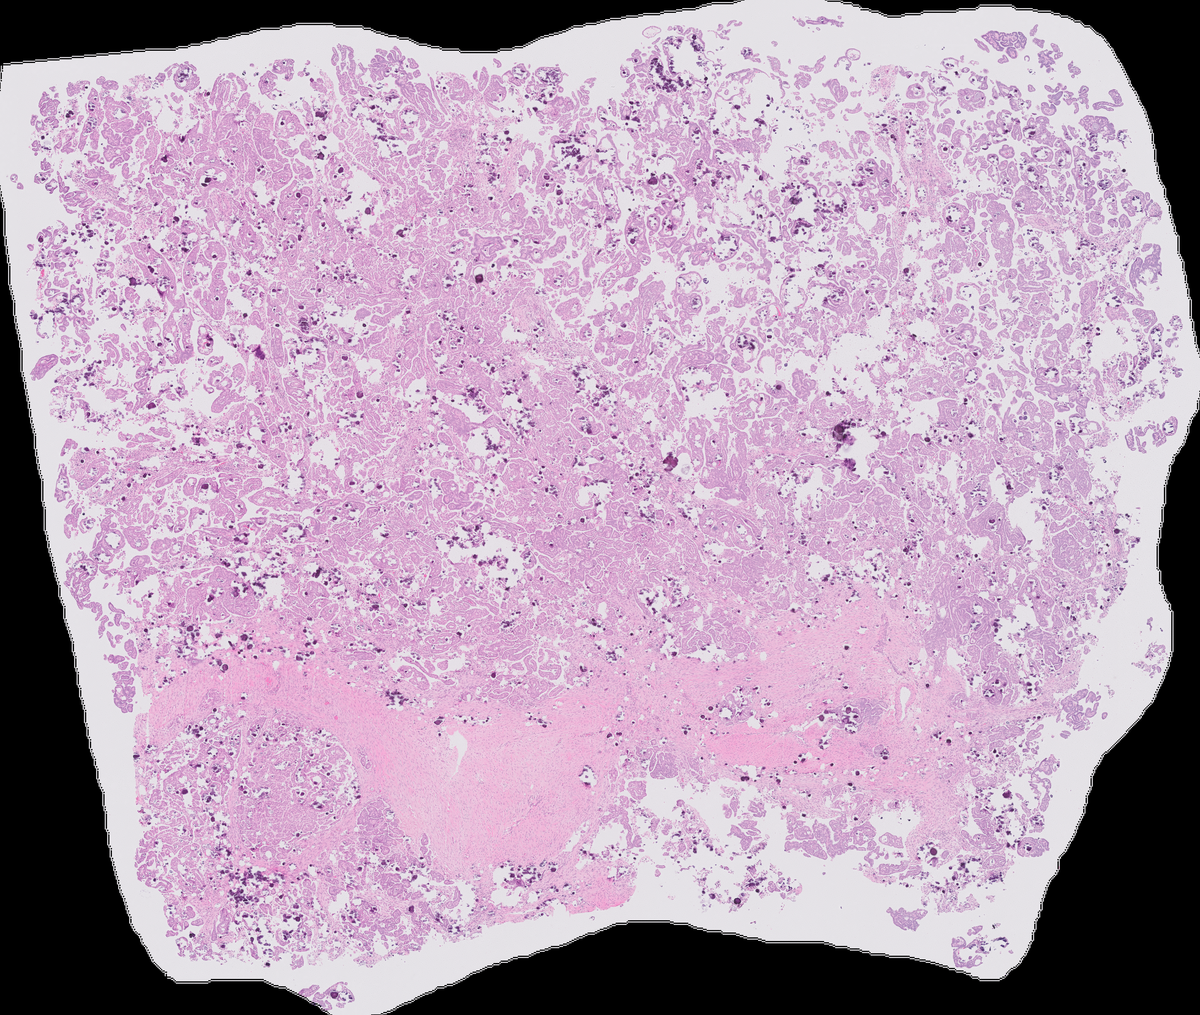
\includegraphics[width=\linewidth]{figures/dataset/wsi_11557_thumbnail.png}}
    \hfill
    \subcaptionbox{Máscara RGB no exhaustiva.\label{fig:wsi-11557-mascara}}[0.315\linewidth]{%
      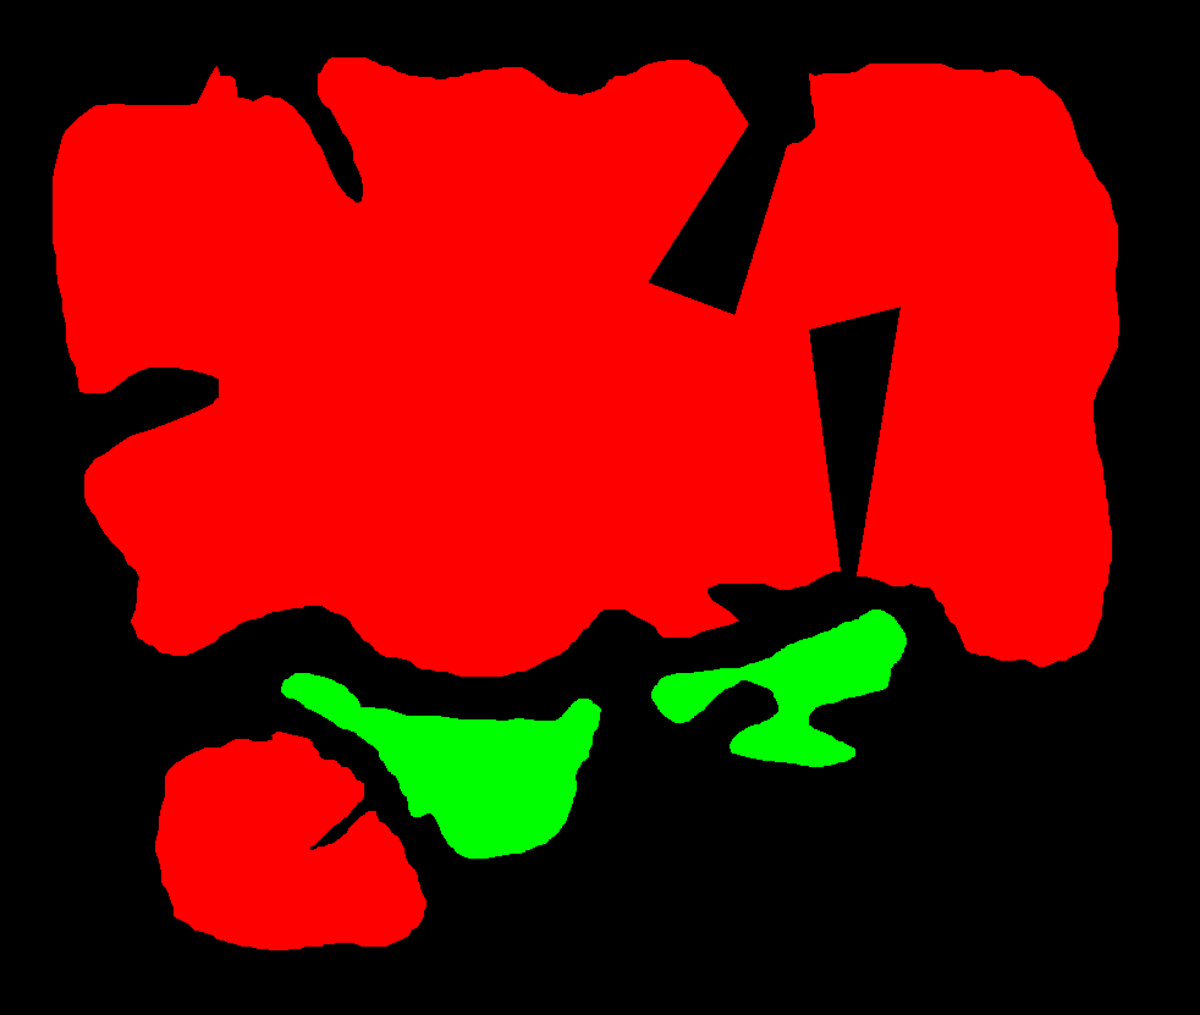
\includegraphics[width=\linewidth]{figures/dataset/wsi_11557_mask.png}}
    \hfill
    \subcaptionbox{Celdas elegibles de $256\times256$.\label{fig:wsi-11557-overlay}}[0.315\linewidth]{%
      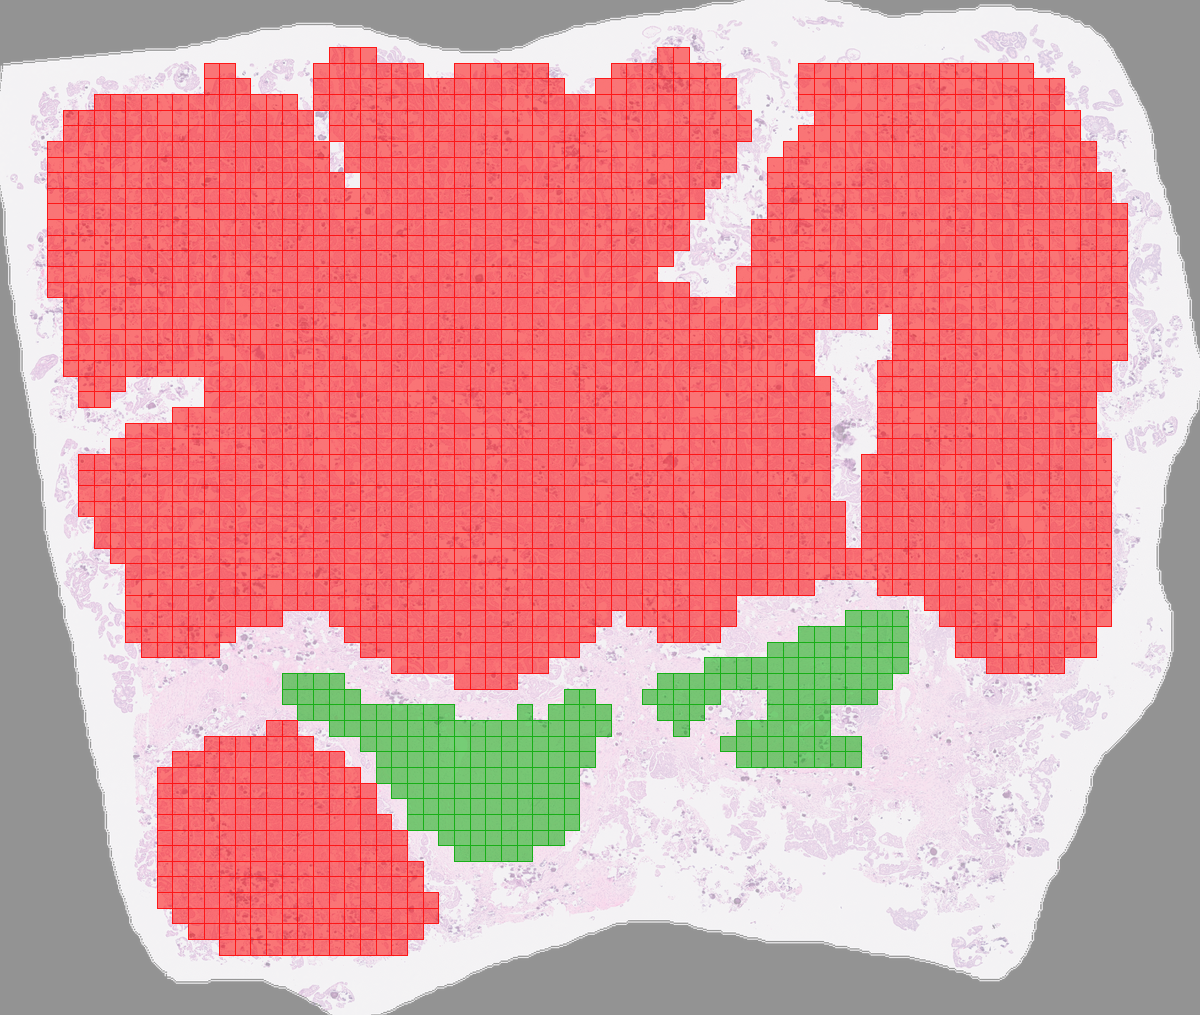
\includegraphics[width=\linewidth]{figures/dataset/wsi_11557_patch_overlay.png}}
    \caption{Ejemplo real de la segmentación de WSI a resolución de parche para
    la lámina 11557. El panel (c) no interpola la máscara: cada rectángulo
    representa una unidad de clasificación que satisface los umbrales de
    cobertura y pureza. En esta lámina aparecen regiones de tumor y estroma,
    pero no de necrosis. Fuente: UBC-OCEAN y sus máscaras
    suplementarias~\cite{ubc_ocean_2023}; composición propia.}
    \label{fig:segmentacion-wsi-esquema}
\end{figure}

El clasificador de tejido empleó tres convoluciones
\(16\rightarrow32\rightarrow64\rightarrow128\), normalización por grupos,
activación GELU, agrupación promedio adaptativa y una capa lineal
\(128\rightarrow3\). Para estudiar eficiencia de etiquetas se entrenaron
modelos independientes con 250, 500, \(1\,000\), \(2\,500\) y \(5\,671\)
parches etiquetados por clase. Los subconjuntos fueron balanceados, anidados y
estratificados por WSI; cada par normal/\(\mathrm{SO}(2)\) partió de los mismos
pesos y recibió los mismos índices en cada época.

\begin{figure}[htbp]
    \centering
    \resizebox{\textwidth}{!}{\begin{tikzpicture}[
    font=\sffamily\scriptsize,
    >={Latex[length=2.2mm]},
    flow/.style={->,thick,draw=black!65},
    common/.style={
        draw=black!70,rounded corners=2pt,align=center,
        minimum height=12mm,minimum width=28mm,fill=orange!18
    },
    patch/.style={
        draw=black!65,rounded corners=2pt,align=center,
        minimum height=12mm,minimum width=31mm,fill=blue!9
    },
    mil/.style={
        draw=black!65,rounded corners=2pt,align=center,
        minimum height=12mm,minimum width=35mm,fill=violet!9
    },
    outputbox/.style={
        draw=black!70,rounded corners=2pt,align=center,
        minimum height=12mm,minimum width=31mm,fill=green!12
    }
]
\node[common] (mu) {Codificador VAE congelado\\
    \(\boldsymbol{\mu}:16\times32\times32\) por parche};

\node[patch,right=11mm of mu,yshift=10mm] (tconv) {Conv + GN + GELU\\
    \(16\to32\to64\to128\)};
\node[patch,right=7mm of tconv] (tpool) {Promedio espacial\\
    + lineal \(128\to3\)};
\node[outputbox,right=7mm of tpool] (tout) {Tumor / estroma / necrosis\\
    por celda seleccionada};

\node[mil,right=11mm of mu,yshift=-15mm] (mconv) {Codificador de parche\\
    \(16\to64\to128\to192\)};
\node[mil,right=7mm of mconv,minimum height=20mm] (local) {
    \(\begin{smallmatrix}
    \circ&\circ&\circ&\circ&\circ\\
    \circ&\circ&\circ&\circ&\circ\\
    \circ&\circ&\bullet&\circ&\circ\\
    \circ&\circ&\circ&\circ&\circ\\
    \circ&\circ&\circ&\circ&\circ
    \end{smallmatrix}\)\quad
    \begin{tabular}{c}2 bloques locales\\radio 2, 6 cabezas\end{tabular}};
\node[mil,right=7mm of local] (summary) {CLS + 16 registros\\
    lectura sigmoidal\\\(\sigma(qk/\sqrt{32}+b-\log N)\)};
\node[mil,below=7mm of summary] (cls) {Atención \emph{softmax}\\
    CLS sobre 17 tokens};
\node[outputbox,right=7mm of cls] (mout) {Diagnóstico WSI\\
    5 subtipos};

\draw[flow] (mu.east) -- ++(5mm,0) |- (tconv.west);
\draw[flow] (tconv) -- (tpool);
\draw[flow] (tpool) -- (tout);
\draw[flow] (mu.east) -- ++(5mm,0) |- (mconv.west);
\draw[flow] (mconv) -- (local);
\draw[flow] (local) -- (summary);
\draw[flow] (summary) -- (cls);
\draw[flow] (cls) -- (mout);

\node[draw=blue!45,dashed,rounded corners=2pt,fit=(tconv)(tpool)(tout),
      inner sep=3mm,label={[font=\sffamily\scriptsize,text=blue!65!black]above:
      Segmentación en cuadrícula dispersa de parches}] {};
\node[draw=violet!45,dashed,rounded corners=2pt,fit=(mconv)(local)(summary)(cls)(mout),
      inner sep=3mm,label={[font=\sffamily\scriptsize,text=violet!65!black]below:
      Clasificación mediante aprendizaje de instancias múltiples}] {};
\end{tikzpicture}
}
    \caption{Arquitecturas supervisadas aplicadas sobre la media posterior
    congelada. La rama superior produce una etiqueta por celda seleccionada de
    la cuadrícula y la rama inferior agrega la bolsa completa para producir el
    diagnóstico de la WSI. Elaboración propia a partir de las implementaciones
    finales.}
    \label{fig:arquitecturas-supervisadas}
\end{figure}

Cada presupuesto se optimizó por un máximo de 30 épocas con AdamW y tasa máxima
de \(1,5\times10^{-3}\). El calentamiento lineal ocupó
\(\lceil0,1S\rceil\) actualizaciones, donde \(S\) es el número de pasos de una
época; correspondió a 1, 2, 3, 6 y 11 actualizaciones para los cinco
presupuestos, respectivamente, y fue seguido por decaimiento coseno. La
selección se hizo por macro-F1 de validación y la parada temprana solo pudo
activarse después de completar diez épocas. En la prueba se evaluaron los
\(31\,572\) parches una sola vez y se reportaron macro-F1 como medida principal,
exactitud balanceada, exactitud, entropía cruzada, métricas por clase y matrices
de confusión.

Esta evaluación no puede considerarse una segmentación exhaustiva: las
etiquetas no cubren toda la extensión de las WSI y las regiones negras o no
pintadas no equivalen a una clase negativa. En consecuencia, los resultados
cuantifican el desempeño en regiones anotadas de alta pureza, mientras que los
mapas sobre la lámina muestran la resolución y el comportamiento espacial del
método sin convertir áreas no anotadas en verdad de referencia.

\subsection{Análisis del espacio latente}

El análisis latente utilizó la media posterior y mantuvo congelados los dos
modelos. Su motivación se apoyó en EQ-VAE, donde se plantea que una respuesta
latente más equivariante frente a transformaciones que preservan el contenido
puede reducir la complejidad de la distribución que deberá aprender un modelo
posterior~\cite{kouzelis_eqvae_2025}. Esta tesis no reprodujo su término de
regularización ni evaluó un generador: tomó de ese trabajo la pregunta
geométrica y la convención de visualizar por PCA la organización espacial del
latente, y la adaptó a dos codificadores entrenados desde cero sobre parches
histopatológicos.

Una primera descripción trató las \(32\times32\) posiciones de cada mapa como
observaciones de 16 variables latentes. Tras excluir las esquinas afectadas
por la rotación interpolada, se ajustó PCA y se llevaron sus tres componentes
principales a RGB. Se produjeron dos vistas complementarias: una escala
independiente por parche, útil para revelar estructura interna, y un ajuste
común por modelo sobre los 25 parches, apropiado para acompañar la comparación
numérica. Debido a la ambigüedad de signos, ejes y escalas de PCA, los colores
no se compararon como si fueran canales alineados entre modelos. Además, se
calculó la RMS relativa de aristas locales

\begin{equation}
    r_{\mathrm{arista}}
    =\frac{
        \sqrt{\operatorname{media}_{(u,v)\in\mathcal{E}}
        \lVert\boldsymbol{\mu}_u-\boldsymbol{\mu}_v\rVert_2^2}
    }{
        \sqrt{\operatorname{media}_{u}
        \lVert\boldsymbol{\mu}_u-\overline{\boldsymbol{\mu}}\rVert_2^2}
    },
    \label{eq:rms-aristas-latentes}
\end{equation}

donde \(\mathcal{E}\) contiene las parejas horizontales y verticales vecinas.
El numerador mide cambios locales y el denominador, la variación espacial
centrada del mismo parche. Un valor menor indica un campo localmente menos
rugoso, pero no implica por sí solo mayor calidad ni equivarianza, pues también
puede resultar de una representación suavizada o colapsada. Los colores se
normalizaron por modelo y, por tanto, sirvieron para estudiar organización
espacial interna, no para alinear canales entre modelos entrenados por separado.

La respuesta a rotaciones se evaluó sobre 25 parches fijos provenientes de 16
WSI. Para cada parche se generó una órbita de 360 vistas, con pasos de un
grado, mediante una transformación bilineal cuya orientación se validó con
patrones asimétricos. Se conservaron controles exactos a 90, 180 y 270 grados.
Cada vista se codificó por separado y la media posterior se restringió a un
disco central de radio 14, equivalente a 616 celdas y 9\,856 valores por
ángulo. Sobre las 360 observaciones se ajustó un PCA independiente para cada
modelo y parche; sus dos primeras coordenadas sirvieron para dibujar la órbita,
no para comparar escalas entre paneles. Sobre la trayectoria completa se
midieron longitud, diferencias de primer y segundo orden, linealidad local,
curvatura, concentración espectral armónica y dimensión de subespacios
tangentes. Las rotaciones de un grado permitieron estudiar continuidad local,
mientras los cuartos de vuelta evitaron interpolación y actuaron como controles
exactos de la cuadrícula.

En el VAE-\(\mathrm{SO}(2)\) también se evaluó directamente la ley de
transformación de los campos internos \(F_1\). Para el posterior escalar se
comparó \(E(R_\theta\mathbf{x})\) con la rotación espacial prescrita de
\(E(\mathbf{x})\), y se estudió la reconstrucción después de transformar o
canonizar el latente. Los ángulos son mediciones repetidas de los mismos
parches y no muestras biológicas independientes. El análisis funcional de la
geometría latente está planificado, pero aún no se ha ejecutado y permanece
fuera del alcance de esta versión. Hasta contar con resultados trazables no se
adelantan conclusiones sobre factorización, topología o una acción global
aprendida.

\section{Análisis estadístico}

Las comparaciones se definieron de forma pareada: una misma lámina, parche o
presupuesto produjo una observación para cada representación. Cuando la medida
principal fue calculada por parche, la incertidumbre no se obtuvo
remuestreando parches como si fueran independientes. Se aplicaron \(10\,000\)
réplicas de bootstrap por conglomerados de WSI y se conservaron las mismas
multiplicidades para ambos modelos.

En reconstrucción, las 23 WSI se remuestrearon sin estratificar. Para
diagnóstico se remuestrearon las WSI dentro de cada subtipo. Para tejido
se usaron estratos definidos por la disponibilidad de las tres clases y se
transportaron todos los parches de cada WSI seleccionada. La familia principal
de tejido incluyó las cinco diferencias de macro-F1 y el área normalizada bajo
la curva de macro-F1 frente al logaritmo del número de etiquetas; sus
intervalos simultáneos controlaron la lectura aislada de un presupuesto.

Los intervalos del 95\% describen la incertidumbre asociada con las WSI
observadas. No incorporan variación entre inicializaciones, otros selectores de
parches ni otros conjuntos de datos. Los análisis sobre los 25 parches fijos se
trataron como descripciones de ese conjunto y se informaron mediante medianas,
conteos favorables y controles predefinidos, sin denominarlos pruebas de
significancia poblacional.

\section{Reproducibilidad y trazabilidad}

El código, las configuraciones, las especificaciones de datos y los protocolos se
mantuvieron versionados en el repositorio del experimento. Cada población
lógica se vinculó con un manifiesto ordenado por identidad de WSI y coordenada;
los trabajos remotos registraron sus entradas, entorno de ejecución, salidas y
metadatos de descarga. Los puntos de control finales y las figuras incluidas en
este documento se conservaron sin modificaciones y su procedencia se verificó
antes de redactar resultados. Los identificadores técnicos necesarios para
repetir esa verificación permanecen en los manifiestos del repositorio.

Las particiones, los presupuestos de etiquetas y los criterios de selección se
fijaron antes de abrir la prueba sellada. La inferencia de prueba se ejecutó sin
etiquetas y sus predicciones se sellaron antes de efectuar la unión local con
la verdad de referencia. Esta separación permitió verificar que la prueba no se
utilizó para ajustar modelos, escoger puntos de control o repetir una
configuración desfavorable.

\section{Consideraciones éticas y manejo de datos}

La investigación se limitó al análisis secundario de imágenes y metadatos
distribuidos públicamente para una competencia de investigación. No se
realizaron intervenciones en pacientes, no se modificó la atención clínica y
no se incorporaron nombres, direcciones, teléfonos ni historias clínicas al
repositorio de trabajo. Los artefactos derivados se identificaron por el
código de la lámina y se emplearon exclusivamente para los objetivos
computacionales descritos.

Se respetaron las condiciones de uso de la fuente y no se intentó
reidentificar a los participantes. Los resultados se presentan como evidencia
experimental sobre el conjunto analizado y no como un dispositivo diagnóstico
ni como recomendación clínica. La determinación institucional de aprobación,
exención o clasificación ética que corresponda deberá constar en los anexos
administrativos antes del depósito final; las referencias generales a la
Declaración de Helsinki y a las pautas CIOMS del plan no sustituyen esa
constancia específica.
